% Settings for the default beamer theme
\documentclass[english, aspectratio=169]{beamer}
\usepackage[T1]{fontenc}
\usepackage[utf8]{inputenc}
\usepackage{adjustbox}
\usepackage{tabularx}
\usepackage{listings}
\usepackage{graphicx}
\usepackage{array}
\usepackage{babel}
\usepackage[ruled,vlined]{algorithm2e}
\usepackage{blkarray}
\SetAlgorithmName{Algoritmus}{algoritmus}{List of Algorithms}
\setcounter{secnumdepth}{3}
\setcounter{tocdepth}{3}


\makeatletter

\newcommand\makebeamertitle{\frame{\maketitle}}

% (ERT) argument for the TOC
\AtBeginDocument{%
	\let\origtableofcontents=\tableofcontents
	\def\tableofcontents{\@ifnextchar[{\origtableofcontents}{\gobbletableofcontents}}
	\def\gobbletableofcontents#1{\origtableofcontents}
}

% Theme settings
\usetheme{Frankfurt}
\usecolortheme{default}
\usefonttheme[onlymath]{serif}

% Template settings
\setbeamertemplate{navigation symbols}{}
\setbeamertemplate{blocks}[rounded][shadow=false]
\setbeamertemplate{title page}[default][colsep=-4bp, rounded=true, shadow=false]
\makeatother

% Custom color definitions
\definecolor{lightgrey}{gray}{0.95}
\definecolor{DarkerGreen}{RGB}{0,85,0} % Adjust the RGB values as needed

% Use the newly defined color in Beamer theme elements
\setbeamercolor{structure}{fg=DarkerGreen} % Changes basic structural elements to Darker Green
\setbeamercolor{title in head/foot}{bg=DarkerGreen} % Changes the title in header/footer to Darker Green

% Definitions for program code sections
\lstset{
	language=bash,
	basicstyle=\ttfamily\footnotesize, % Monospace font
	backgroundcolor=\color{lightgrey}, % Background color
	frame=single, % Frame around the code
	keywordstyle=\color{black}, % Keywords color
	commentstyle=\color{black}, % Comments color
	stringstyle=\color{red}, % Strings color
	showstringspaces=false, % Do not show spaces in strings
	breaklines=true, % Automatically break long lines
}

\lstset{
	language=python,
	basicstyle=\ttfamily\scriptsize, % Basic font style
	keywordstyle=\bfseries\color{blue}, % Keywords in bold and blue
	stringstyle=\color{red}, % Strings in red
	commentstyle=\color{green!50!black}, % Comments in green
	showstringspaces=false, % Do not show spaces in strings
	numbers=left, % Line numbers on the left
	numberstyle=\tiny\color{gray}, % Line number style
	stepnumber=1, % Line number step
	numbersep=5pt, % Distance of line numbers from code
	frame=single, % Frame around the code
	rulecolor=\color{black}, % Frame color
	tabsize=2, % Tab size
	breaklines=true, % Automatic line breaking
	breakatwhitespace=false, % Break lines at whitespace
	captionpos=b, % Caption position
	escapeinside={\%*}{*)}, % Escape to LaTeX
	morekeywords={self}, % Additional keywords
    literate={á}{{\'a}}1
    	{é}{{\'e}}1
		{í}{{\'i}}1
		{ó}{{\'o}}1
		{ú}{{\'u}}1
		{ő}{{\H{o}}}1
		{ű}{{\H{u}}}1
		{Á}{{\'A}}1
		{É}{{\'E}}1
		{Í}{{\'I}}1	
		{Ó}{{\'O}}1	
		{Ú}{{\'U}}1
		{Ő}{{\H{O}}}1
		{Ű}{{\H{U}}}1
       	{Ö}{{\"O}}1
		{Ü}{{\"U}}1
		{ö}{{\"o}}1
		{ü}{{\"u}}1
}

\begin{document}

% Title page
\section{Bevezetés}
\title[]{Adatbányászat a Gyakorlatban}
\subtitle{3. Gyakorlat: Dash diagramok}
\author[Kuknyó Dániel]{Kuknyó Dániel\\Budapesti Gazdasági Egyetem}
\date{2024/25\\1.félév}
\makebeamertitle

% Table of contents slide
\begin{frame}
\tableofcontents{}
\end{frame}

% Table of contents of the current section
\begin{frame}
\tableofcontents[currentsection]
\end{frame}

\begin{frame}[fragile]{\texttt{A Figure objektum}}
	\begin{columns}
		\begin{column}{.5\textwidth}
			A Plotly-ban a \texttt{Figure} objektum egy magasszintű adatstruktúra, amely egyesíti a diagram adatait és elrendezését egyetlen objektumban. Olyan attribútumokat tartalmaz, mint a \texttt{data} és \texttt{layout}.
			\vspace{0.2cm}
			\begin{lstlisting}[language=python]
import plotly.graph_objects as go

fig = go.Figure()
			\end{lstlisting}
		\end{column}
		\begin{column}{.5\textwidth}
			\begin{center}
				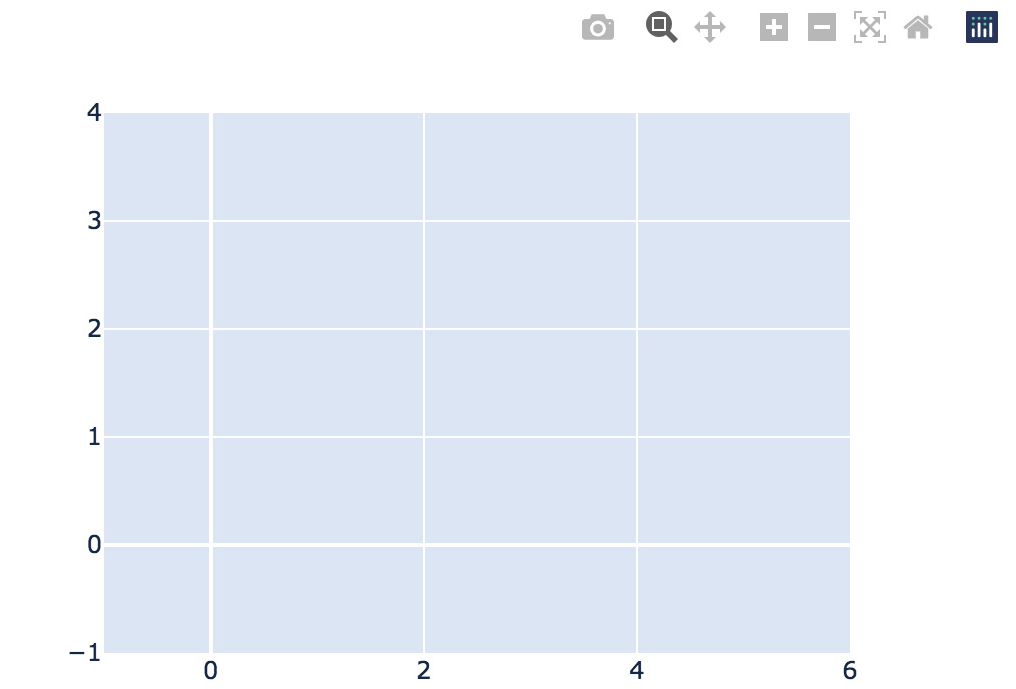
\includegraphics[width=5cm, height=5cm, keepaspectratio]{images/plots_1.png}
			\end{center}
		\end{column}
	\end{columns}
\end{frame}

\begin{frame}{\texttt{Figure} objektumok attribútumai}
	\begin{columns}
		\begin{column}{.5\textwidth}
			\begin{block}{\texttt{data}}
				 Ez az attribútum tartalmazza a diagramon megjelenítendő adatokat. Ez egy lista, amely különböző nyomokat (\texttt{trace}) tartalmaz.
			\end{block}
			\vspace{.3cm}
			\begin{block}{\texttt{trace}}
				Egy \texttt{trace} vagy nyom egy adatcsoportot képvisel a diagramon belül. Minden nyomnak megvan a maga típusa (pl. kör, szórás, oszlop) és különböző tulajdonságokkal rendelkezik, mint az $x$ és $y$ tengely értékei, színek, név stb...
			\end{block}
		\end{column}
		\begin{column}{.5\textwidth}
			\begin{block}{\texttt{layout}}
				Ez az attribútum határozza meg a diagram elrendezését és stílusát. Ide tartoznak a tengelyek címkéi, a diagram címe, a háttérszínek, a margók, a legendák és egyéb vizuális elemek. A \texttt{layout} attribútum egy szótár, amely különböző kulcs-érték párokat tartalmaz.
			\end{block}
		\end{column}
	\end{columns}
\end{frame}

\begin{frame}[fragile]{A \texttt{data} attribútum}
	\begin{columns}
		\begin{column}{.6\textwidth}
			A \texttt{Figure} objektumot a \texttt{plotly.graph\_objects} könyvtár tartalmazza. Példányosítás után az \texttt{add\_scatter()} függvény meghívásával hozzáadódik egy új nyom a vászonhoz. A nyom az $x$ és $y$ koordinátákat tartalmazza a pontdiagramhoz. 
			\vspace*{0.3cm}
			\begin{lstlisting}[language=python]
import plotly.graph_objects as go

fig = go.Figure()
fig.add_scatter(x=[1, 2, 3], y=[4, 2, 3])
fig.show()
			\end{lstlisting}		
		\end{column}
		\begin{column}{.4\textwidth}
			\begin{center}
				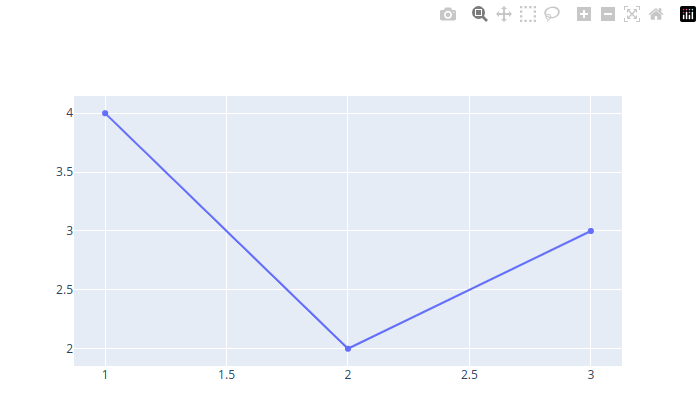
\includegraphics[width=6cm, keepaspectratio]{images/plots_2.png}
			\end{center}
		\end{column}
	\end{columns}
\end{frame}

\begin{frame}[fragile]{A \texttt{layout} attribútum}
	\begin{columns}
		\begin{column}{.5\textwidth}
			A \texttt{layout} attribútum módosítása közvetlen hozzáféréssel lehetséges. Ez egy fastruktúrájú adatszerkezet, ahol az attribútumoknak alárendelt attribútumai vannak.
			\vspace{0.3cm}
			\begin{lstlisting}[language=python]
fig.layout.title = 'The Figure Title'
fig.layout.xaxis.title = 'The X-axis title'
fig.layout.yaxis.title = 'The Y-axis title'				
			\end{lstlisting}
		\end{column}
		\begin{column}{.5\textwidth}
			\begin{center}
				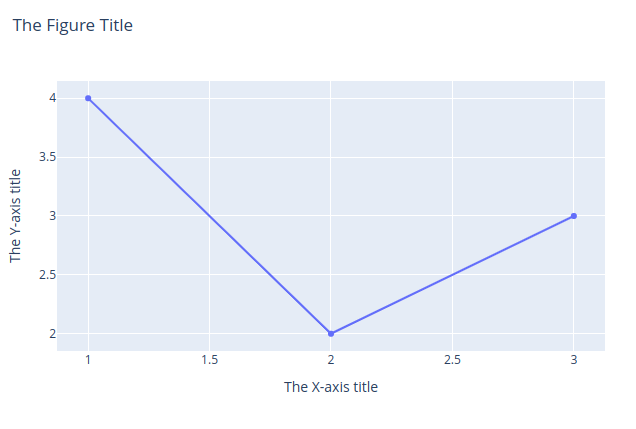
\includegraphics[width=6cm, keepaspectratio]{images/plots_3.png}
			\end{center}
		\end{column}
	\end{columns}
\end{frame}

\section{Grafikonok szerkesztése}

\begin{frame}{}
	\tableofcontents[currentsection]
\end{frame}

\begin{frame}{Grafikon renderelése \texttt{json} formátumba}
	\begin{columns}
		\begin{column}{.4\textwidth}
			A \texttt{show()} függvény több módot is biztosít egy függvény megjelenítésére. Az egyik ilyen a \texttt{fig.show('json')}.\par\smallskip
			Ennek segítségével meg lehet vizsgálni a diagram renderelése közben létrejövő fa struktúrát. 
		\end{column}
		\begin{column}{.6\textwidth}
			\begin{center}
				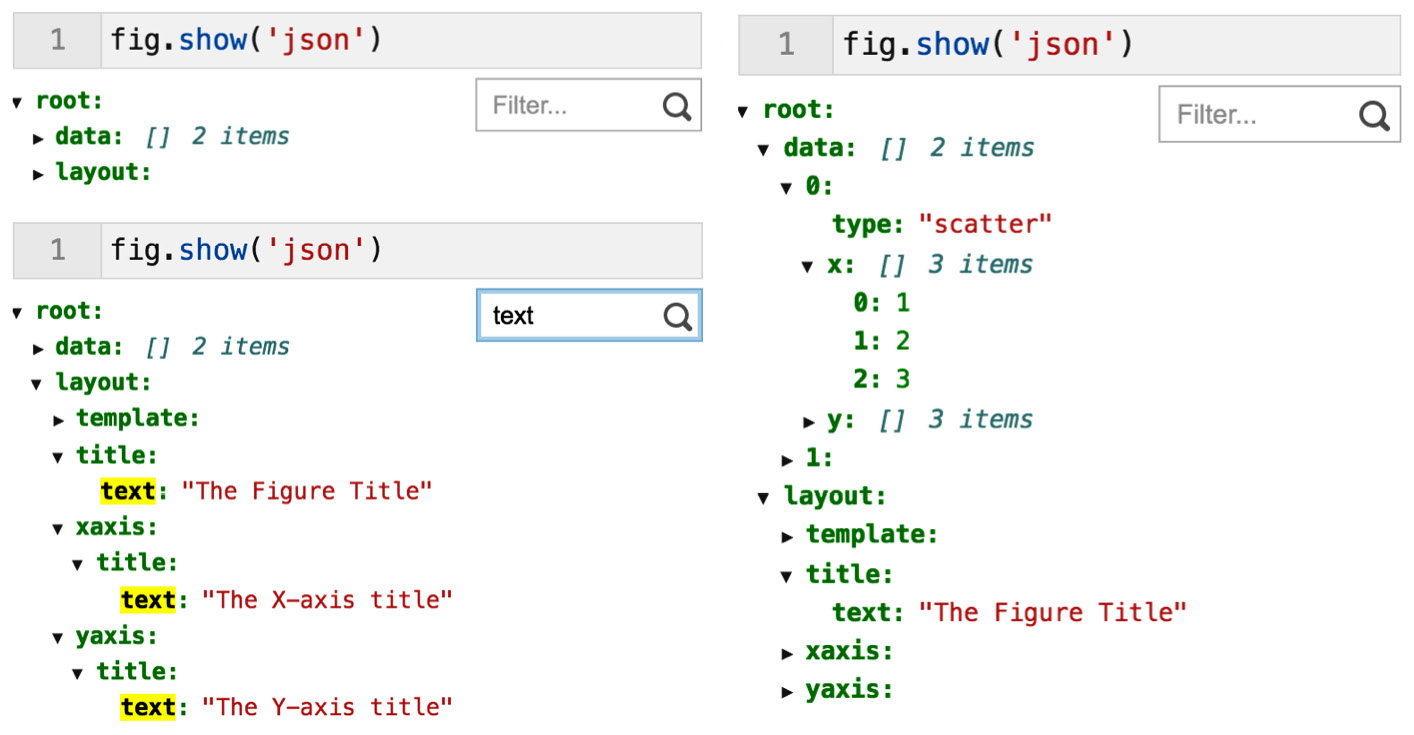
\includegraphics[width=8cm, keepaspectratio]{images/plots_4.png}
			\end{center}
		\end{column}
	\end{columns}
\end{frame}

\begin{frame}[fragile]{Grafikon konfigurálása}
	\begin{columns}
		\begin{column}{.5\textwidth}
			A \texttt{config} paraméter egy \texttt{dict} objektumot vár el, és több tulajdonságát is képes vezérelni a diagramnak:
			\vspace{0.3cm}
			\begin{lstlisting}[language=python]
fig.show(
	config={
		'displaylogo': False,
		'modeBarButtonsToAdd': ['drawrect', 'drawcircle', 'eraseshape']
	}
)
			\end{lstlisting}
		\end{column}
		\begin{column}{.5\textwidth}
			\begin{itemize}
				\item \texttt{displayModeBar}: A teljes menüsáv mutatása, alapértelmezése \texttt{True}
				\item \texttt{responsive}: Változzon-e a diagram mérete a böngésző méretnek megfelelően. Alapértelmezése a \texttt{True}.
				\item \texttt{toImageButtonOptions}: A kép letöltésének alapértelmezett formátumát adja meg. 
				\item \texttt{modeBarButtonsToRemove}: Azon menügombok listája, amiket ne jelenítsen meg a diagram. 
			\end{itemize}
		\end{column}
	\end{columns}
\end{frame}

\begin{frame}[fragile]{Vezérlőkkel összekapcsolt diagramok}
	\begin{columns}
		\begin{column}{.5\textwidth}
			Egy interaktív diagram létrehozása az elrendezésben:
			\begin{lstlisting}[language=python]
app.layout = html.Div([
	dcc.Dropdown(
		id='year_dropdown',
		value='2010',
		options=[{'label': year, 'value': str(year)} for year in range(1974, 2019)]
	),
	dcc.Graph(id='population_chart')
])
			\end{lstlisting}
			A \texttt{Dropdown} komponensben definiálva vannak a lehetséges értékek, és a \texttt{Graph} egy egyedi \texttt{id} adattaggal van ellátva az interaktivitás miatt.
		\end{column}
		\begin{column}{.5\textwidth}
			Az ehhez a diagramhoz tartozó callback függvény a legördülő menü értékét kapja meg paraméterül, az implementációjában leszűri a táblát, majd egy \texttt{Figure} objektumot térít vissza, ami felülírja a \texttt{population\_chart} \texttt{figure} attribútumát:
			\begin{lstlisting}[language=python]
@app.callback(
	Output('population_chart', 'figure'),
	Input('year_dropdown', 'value')
)
def plot_countries_by_population(year):
	year_df = ...
	fig = go.Figure()
	...
	return fig
			\end{lstlisting}
		\end{column}
	\end{columns}
\end{frame}

\begin{frame}{Alkalmazás felépítése interaktív diagrammal (\texttt{app\_v2\_1.py})}
	\begin{columns}
		\begin{column}{.5\textwidth}
			\begin{enumerate}
				\item Pandas importálása, és a szegénységi adatokat tartalmazó fájl megnyitása. 
				\item Régiók kizárása az adatkészletből, hogy csak országok maradjanak.
				\item Egy \texttt{DataFrame} létrehozása, amely csak az országok teljes népességét tartalmazza. 
				\item Egy legördülő menü segítségével ki lehet választani az évet, amely leszűri az adathalmazt, hogy az abból az évből legnépesebb országokat reprezentálja.
				\item Oszlopdiagram létrehozása, amely a legnépesebb országokat tartalmazza. 
			\end{enumerate}
		\end{column}
		\begin{column}{.5\textwidth}
			\begin{center}
				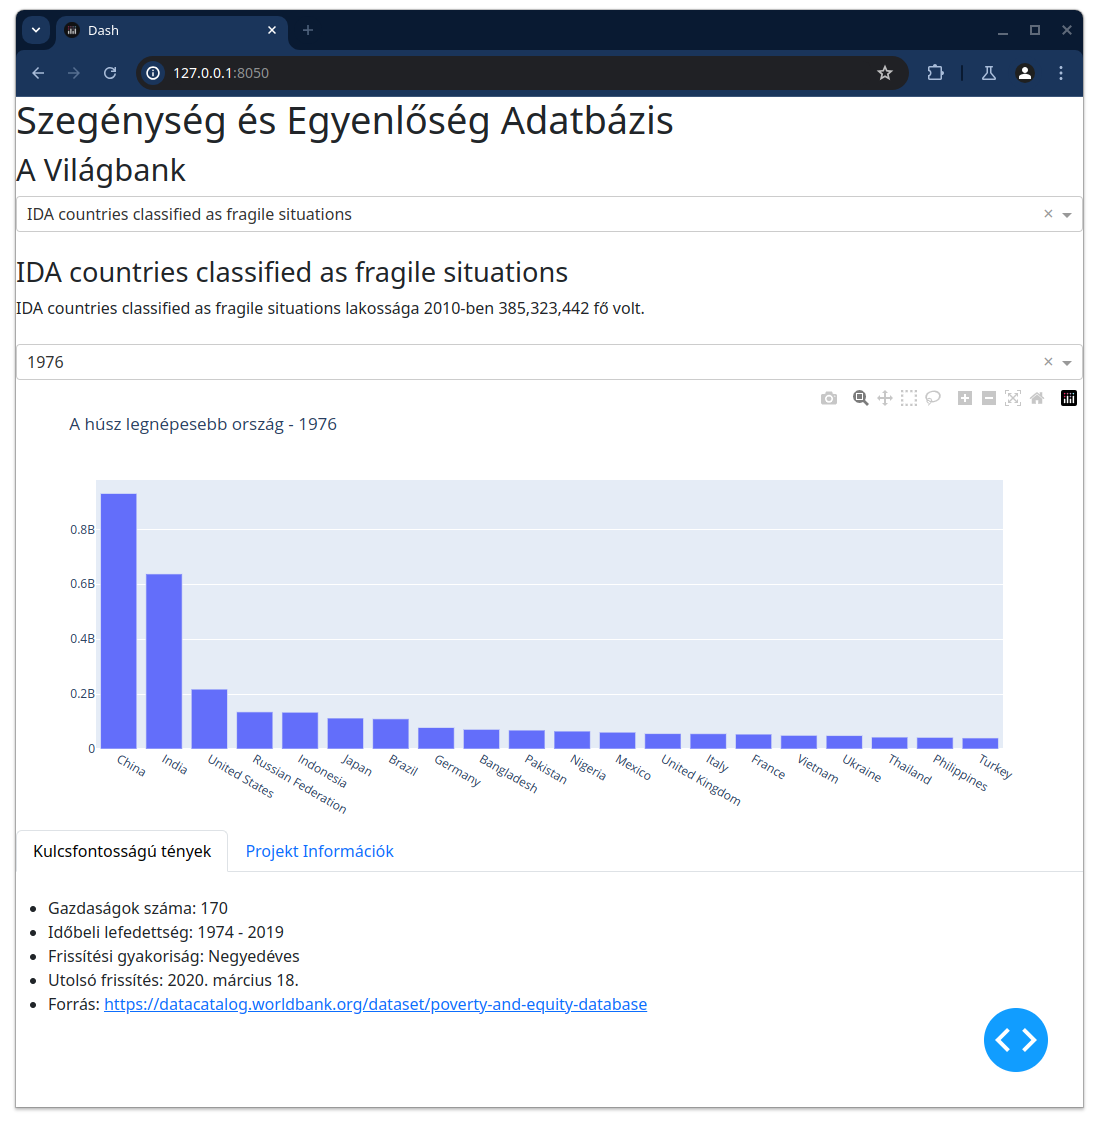
\includegraphics[width=7cm, height=7cm, keepaspectratio]{images/plots_5.png}
			\end{center}
		\end{column}
	\end{columns}
\end{frame}

\begin{frame}{Dash vizuális debugger}
	\begin{columns}
		\begin{column}{.5\textwidth}
			A vizuális debugger a Dash-ben egy eszköz, amely segít a fejlesztőknek nyomon követni és hibakeresni a Dash alkalmazásaikat. A vizuális debugger lehetővé teszi, hogy valós időben lássuk az alkalmazás állapotát, a komponensek közötti adatáramlást és az eseményeket:
			\begin{itemize}
				\item Komponensek hierarchiája
				\item Állapot és tulajdonságok
				\item Események és változások
				\item Hibák és figyelmeztetések
			\end{itemize}
		\end{column}
		\begin{column}{.5\textwidth}
			\begin{center}
				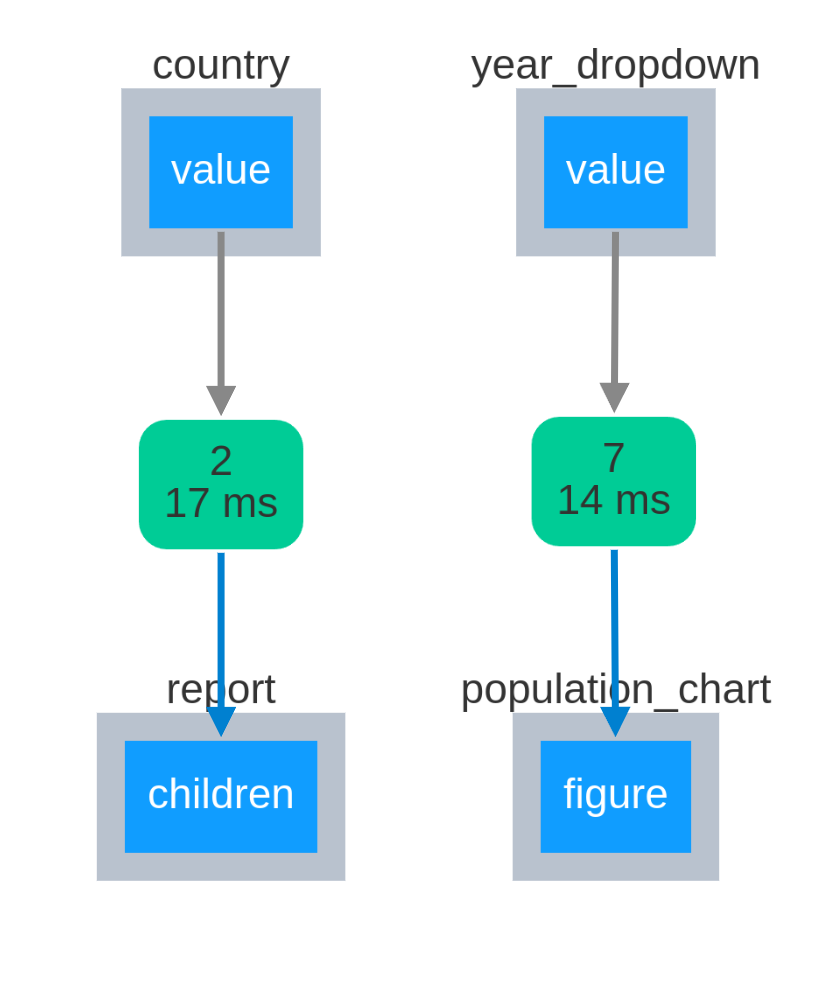
\includegraphics[width=7cm, height=6cm, keepaspectratio]{images/plots_6.png}
			\end{center}
		\end{column}
	\end{columns}
\end{frame}

\begin{frame}[fragile]{Diagram témák szerkesztése}
	\begin{columns}
		\begin{column}{.5\textwidth}
			A diagramok témájának szerkesztése nagyon sok időt megspórolhat, és egy általános megoldást nyújt arra, hogy minden diagram témáját egyszerre lehessen változtatni.\par\smallskip
			Ez a \texttt{layout} alatt a \texttt{template} attribútum módosításával érhető el. 
			\begin{lstlisting}[language=python]
fig.layout.template = template_name
			\end{lstlisting}	
		\end{column}
		\begin{column}{.5\textwidth}
			\begin{center}
				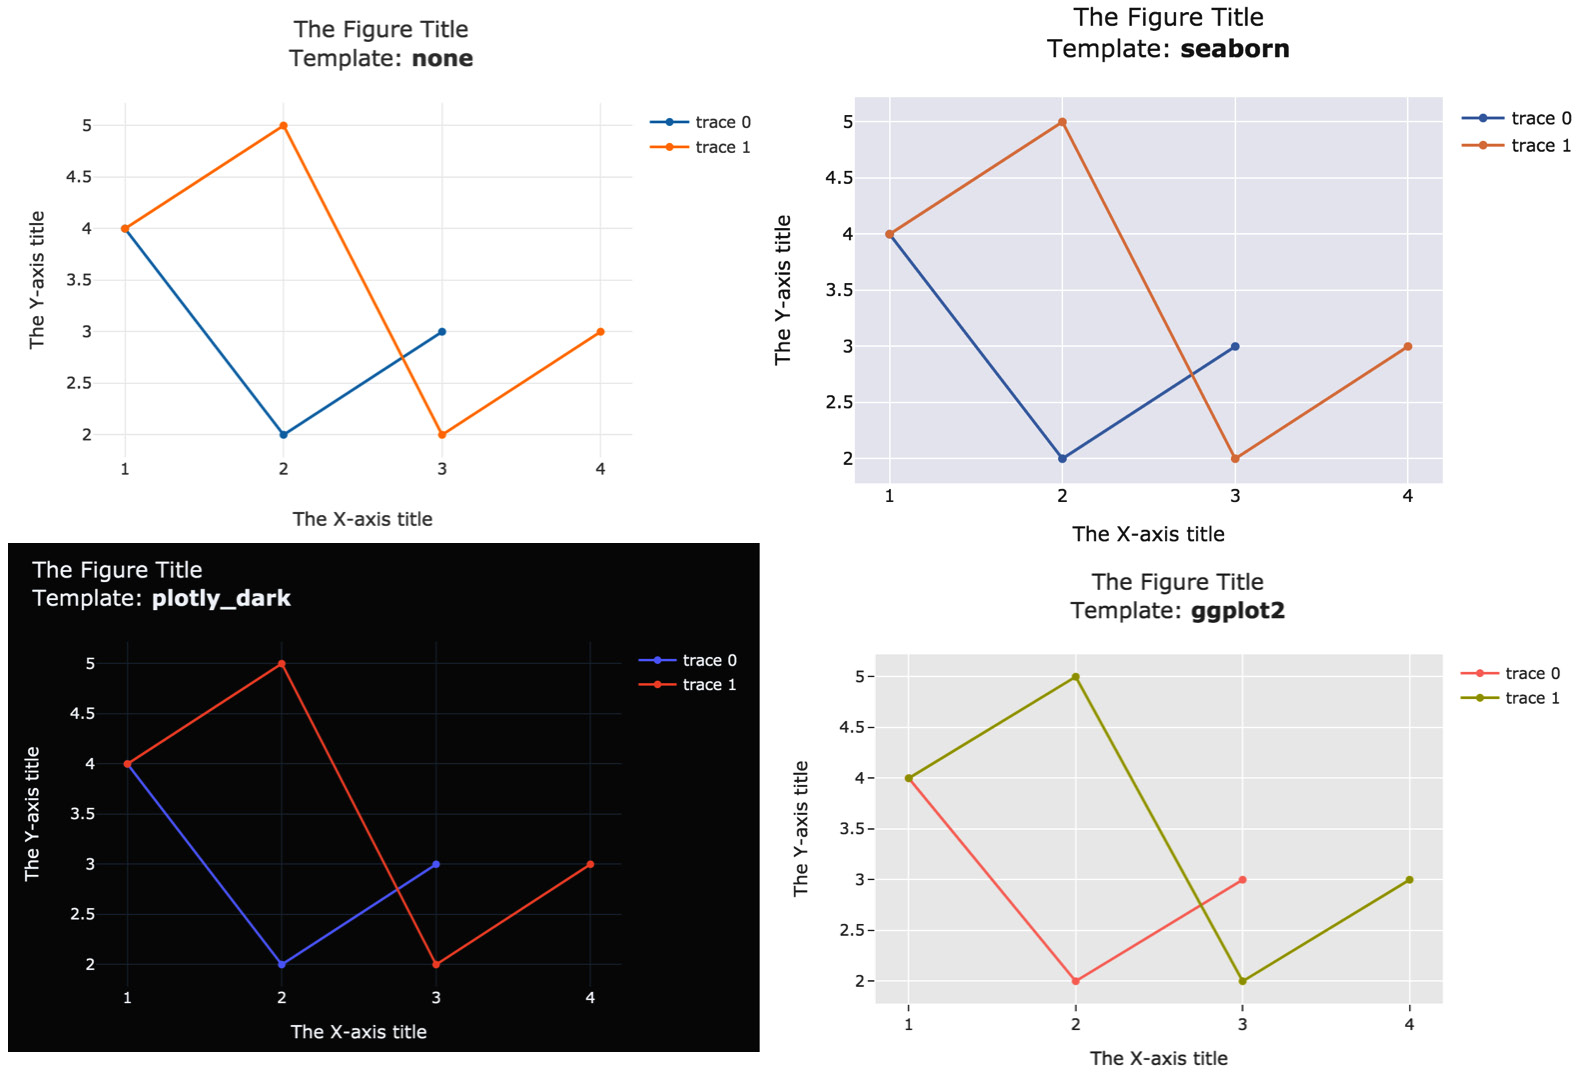
\includegraphics[width=7cm, height=7cm, keepaspectratio]{images/plots_7.png}
			\end{center}
		\end{column}
	\end{columns}
\end{frame}

\section{Plotly express}

\begin{frame}{}
	\tableofcontents[currentsection]
\end{frame}

\begin{frame}[fragile]{Példa adathalmaz definiálása}
	A következőkben a következő egyszerű adattáblával készült diagramok lesznek láthatók:
	\begin{columns}
		\begin{column}{.4\textwidth}
			\begin{lstlisting}[language=python]
df = pd.DataFrame({
	'numbers': [1, 2, 3, 4, 5, 6, 7, 8],
	'colors': ['blue', 'green', 'orange', 'yellow', 'black', 'gray', 'pink', 'white'],
	'floats': [1.1, 1.2, 1.3, 2.4, 2.1, 5.6, 6.2, 5.3],
	'shapes': ['rectangle', 'circle', 'triangle', 'rectangle', 'circle', 'triangle', 'rectangle', 'circle'],
	'letters': list('AAABBCCC')
})
			\end{lstlisting}
		\end{column}
		\begin{column}{.6\textwidth}
			\begin{lstlisting}[language=bash]
   numbers  colors  floats     shapes letters
0        1    blue     1.1  rectangle       A
1        2   green     1.2     circle       A
2        3  orange     1.3   triangle       A
3        4  yellow     2.4  rectangle       B
4        5   black     2.1     circle       B
5        6    gray     5.6   triangle       C
6        7    pink     6.2  rectangle       C
7        8   white     5.3     circle       C
			\end{lstlisting}
		\end{column}
	\end{columns}
\end{frame}

\begin{frame}[fragile]{Pontdiagram}
	\begin{columns}
		\begin{column}{.5\textwidth}
			Egy plotly express diagramnak kétféleképpen is át lehet adni az adathalmazt.\par\medskip
			Az első esetben a \texttt{DataFrame} kerül átadásra, és az \texttt{x, y} paraméterek a \texttt{DataFrame} oszlopaira hivatkoznak:
			\begin{lstlisting}[language=python]
px.scatter(data_frame=df, x='numbers', y='floats')
			\end{lstlisting}
			A másik esetben pedig közvetlenül vannak hivatkozva az oszlopok:
			\begin{lstlisting}[language=python]
px.scatter(x=df['numbers'], y=df['floats'])
			\end{lstlisting}
		\end{column}
		\begin{column}{.5\textwidth}
			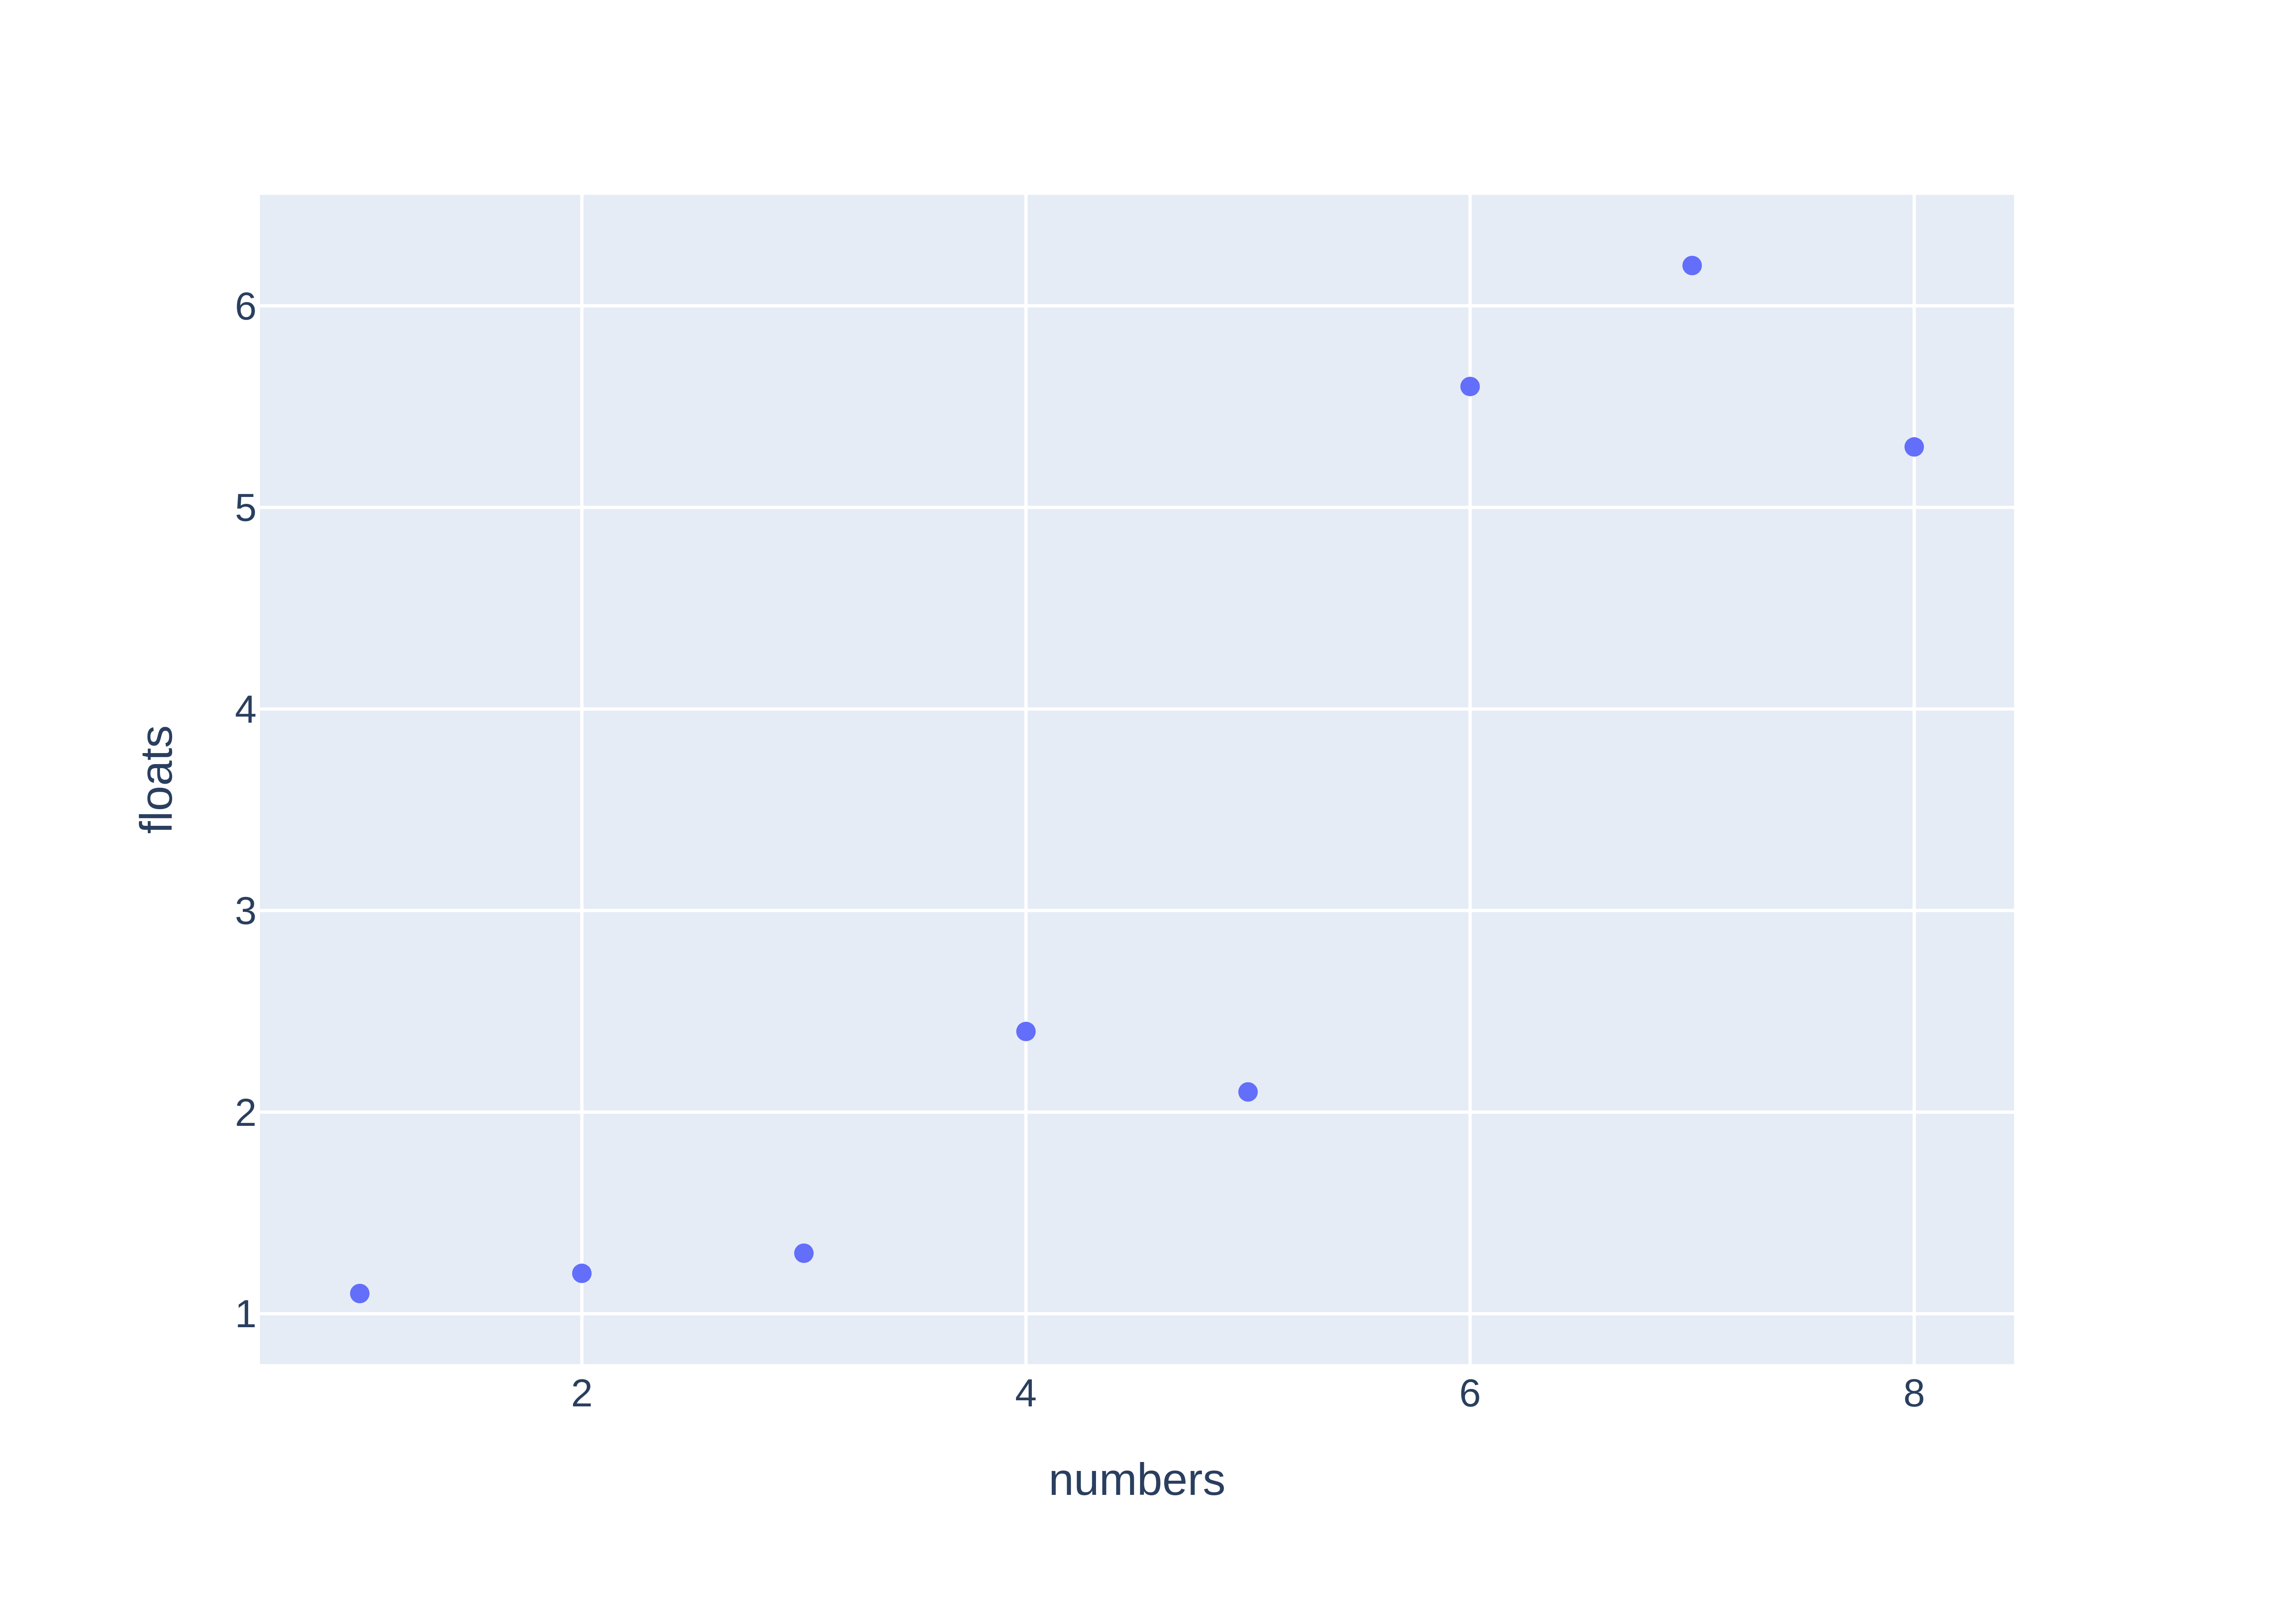
\includegraphics[width=7cm, height=7cm, keepaspectratio]{images/plots_8.png}
		\end{column}
	\end{columns}
\end{frame}

\begin{frame}[fragile]{Pontdiagram kategóriákkal}
	\begin{columns}
		\begin{column}{.5\textwidth}
			Ebben az esetben minden adatosztály egy külön nyomként jelenik meg. 
			\vspace{0.3cm}
			\begin{lstlisting}[language=python]
px.scatter(df, x='numbers', y='floats', color='shapes', symbol='shapes')
			\end{lstlisting}
		\end{column}
		\begin{column}{.5\textwidth}
			\begin{center}
				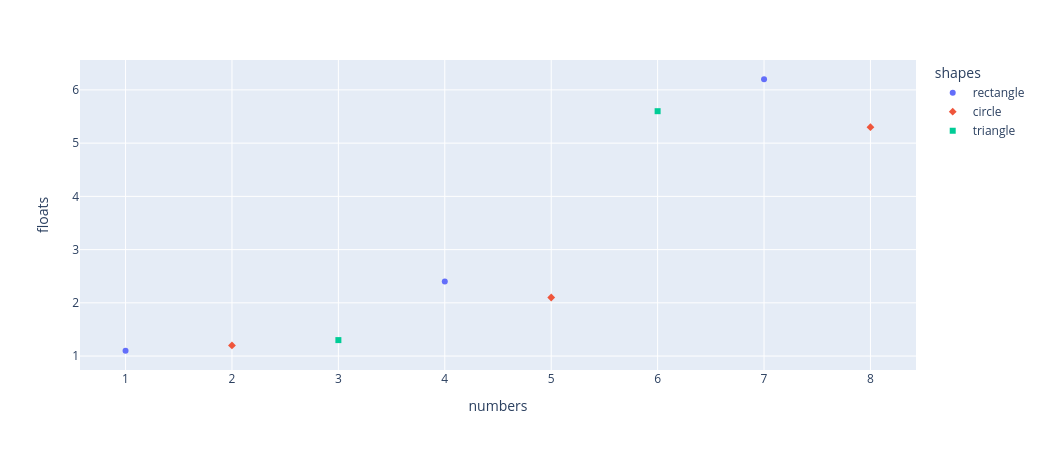
\includegraphics[width=7cm, height=7cm, keepaspectratio]{images/plots_9.png}
			\end{center}
		\end{column}
	\end{columns}
\end{frame}

\begin{frame}[fragile]{Pontdiagram jelölőkkel}
	\begin{columns}
		\begin{column}{.5\textwidth}
			Minden $\left(x,y\right)$ adatpont jelölőjét lehetséges külön állítani. Ezeknek testre lehet szabni a színét, méretét:
			\vspace{0.3cm}
			\begin{lstlisting}
px.scatter(df, x='numbers', y='floats', color='letters', symbol='letters', size=[35] * 8)			
			\end{lstlisting}
		\end{column}
		\begin{column}{.5\textwidth}
			\begin{center}
				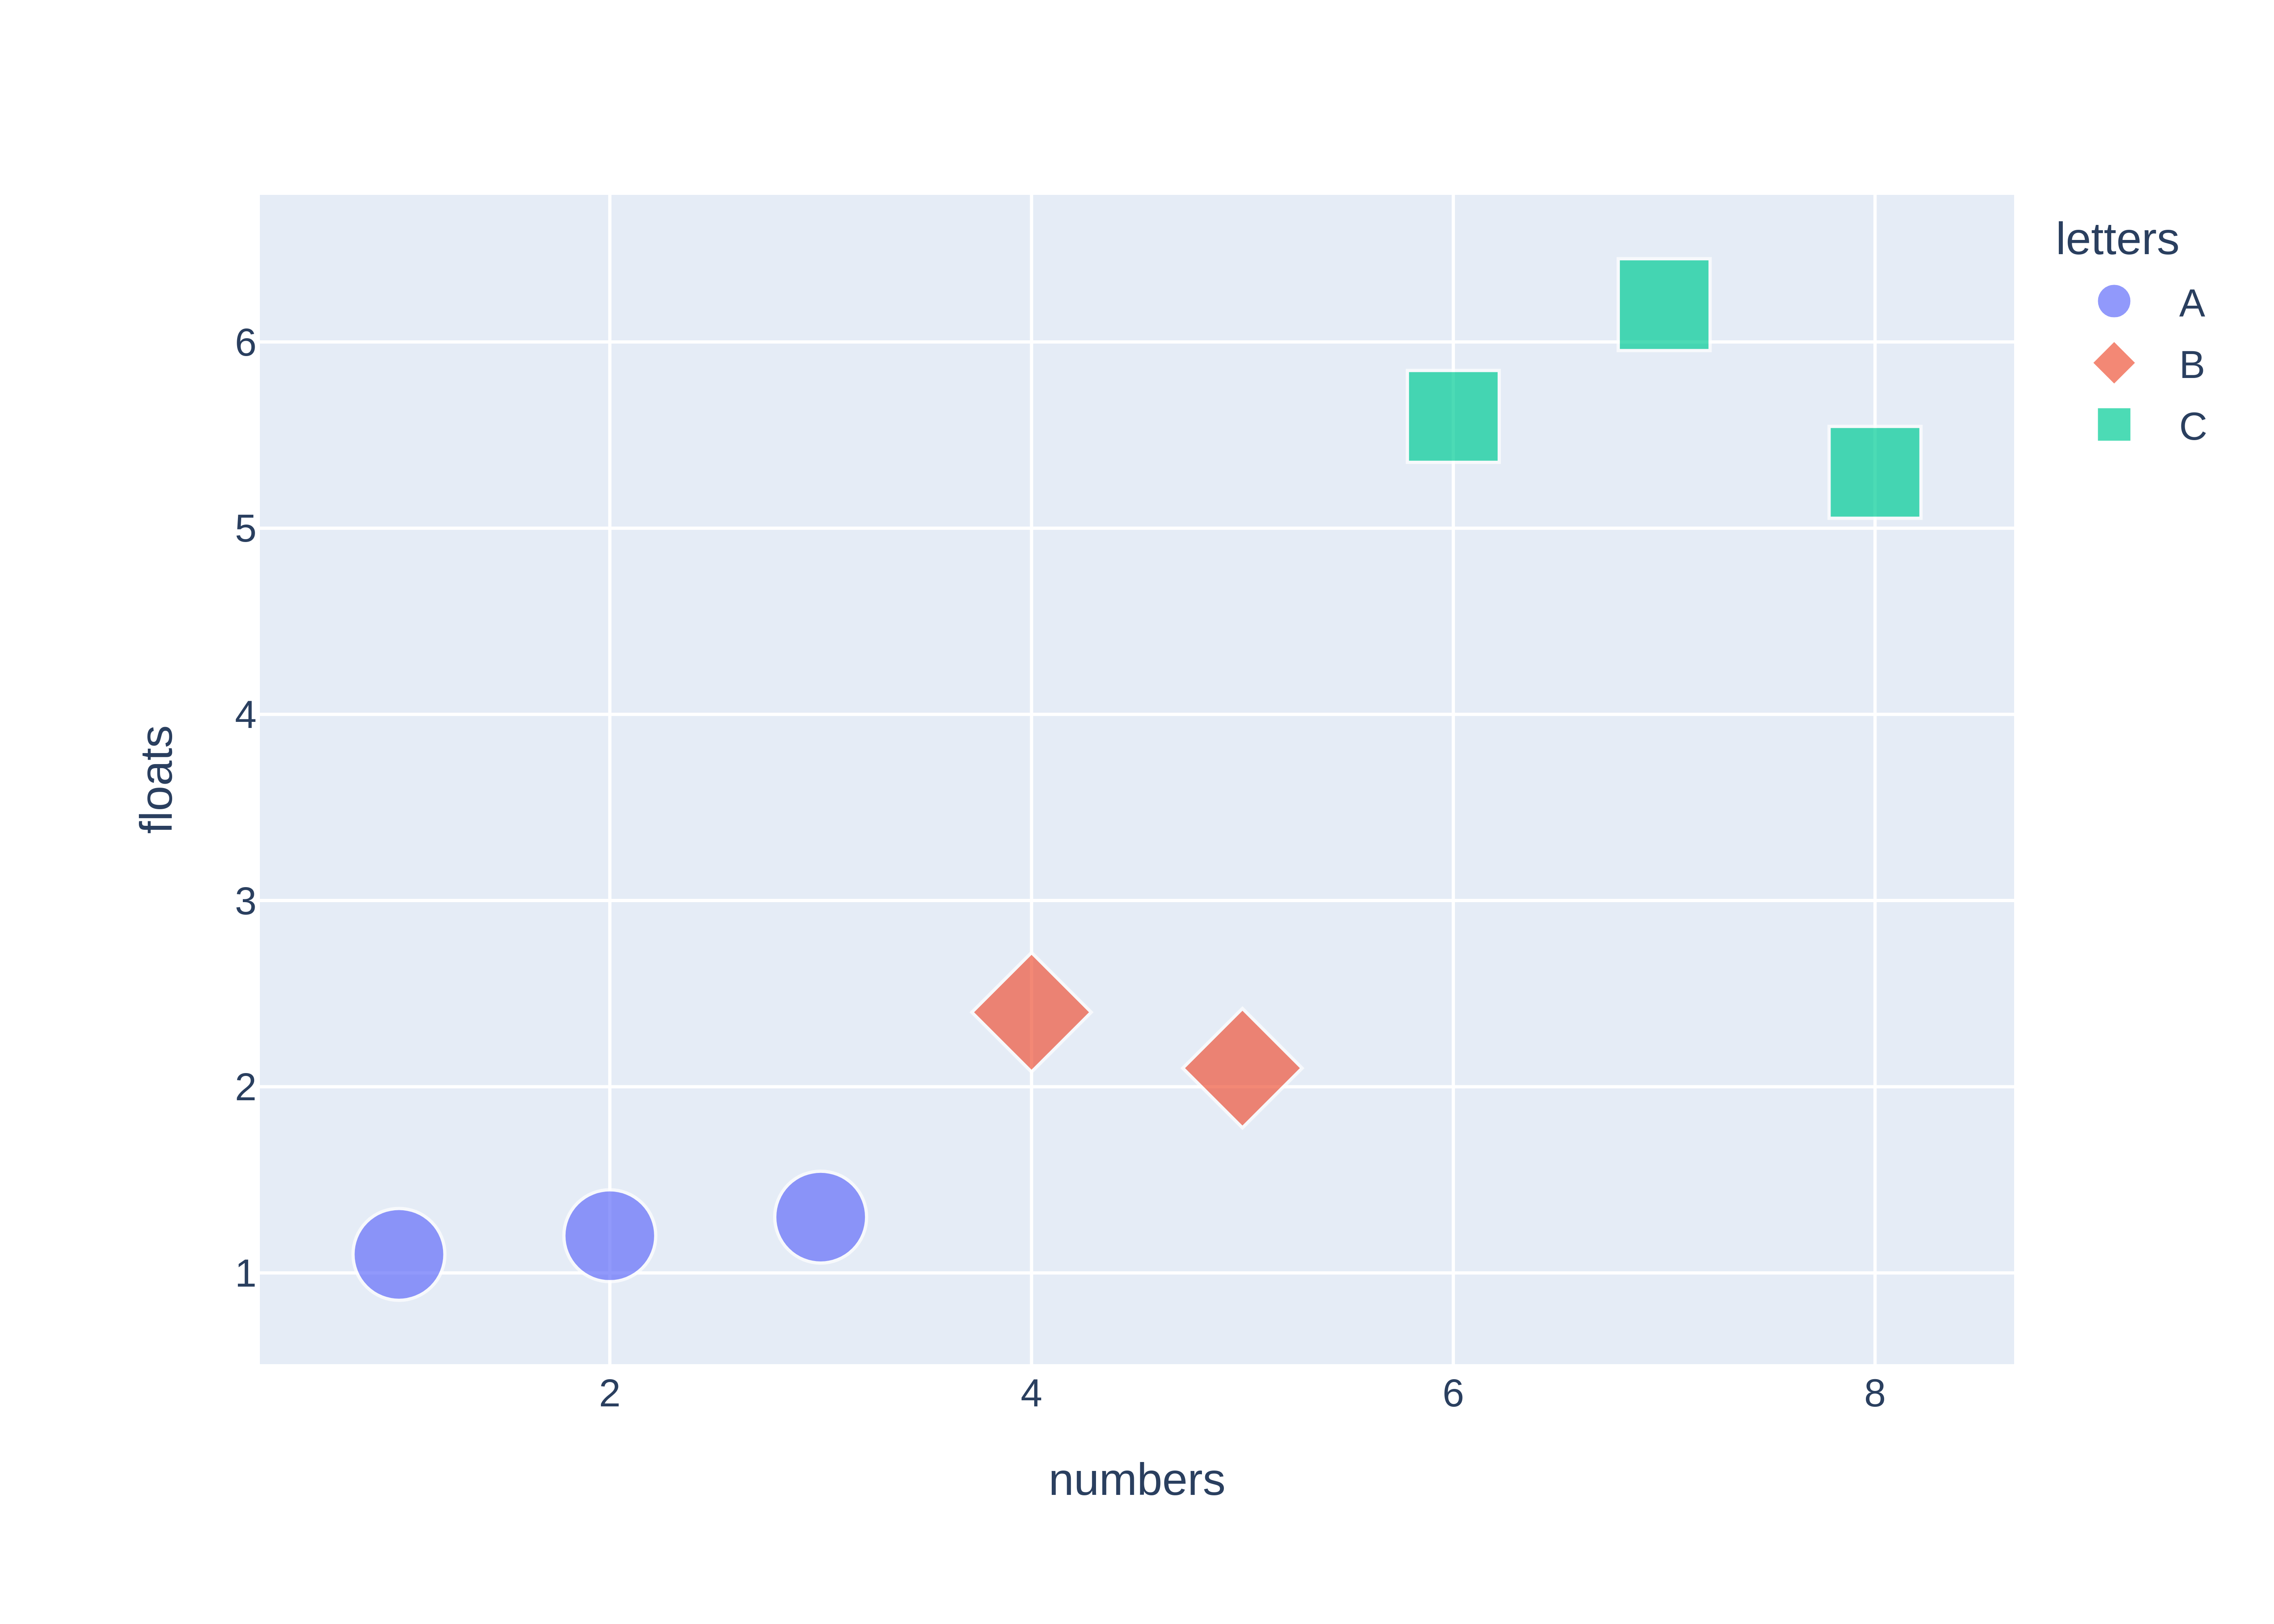
\includegraphics[width=7cm, height=7cm, keepaspectratio]{images/plots_10.png}
			\end{center}
		\end{column}
	\end{columns}
\end{frame}

\begin{frame}[fragile]{Rakott oszlopdiagram}
	\begin{columns}
		\begin{column}{.5\textwidth}
			A rakott oszlopdiagram több oszlopdiagram együttese. Ebben az esetben is minden adatcsoport egy külön nyomként jelenik meg az adatszerkezetben. A csoportosítási változót a \texttt{color} attribútum adja meg. 
			\vspace{0.3cm}
			\begin{lstlisting}[language=python]
px.bar(df, x='letters', y='floats', color='shapes')
			\end{lstlisting}
		\end{column}
		\begin{column}{.5\textwidth}
			\begin{center}
				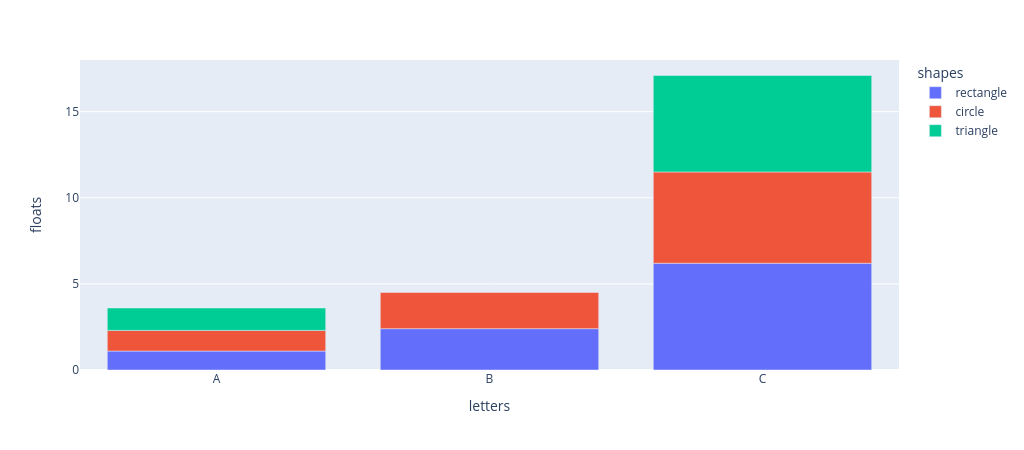
\includegraphics[width=7cm, height=7cm, keepaspectratio]{images/plots_11.png}
			\end{center}
		\end{column}
	\end{columns}
\end{frame}

\begin{frame}[fragile]{Csoportosított oszlopdiagram}
	\begin{columns}
		\begin{column}{.5\textwidth}
			Csoportosítás esetén az adatcsoportok nem egymáson, hanem egymás mellett foglalnak helyet. A csoportosítás attribútuma itt is a \texttt{color}, és a csoportosítási típust a \texttt{barmode=color} adja meg. 
			\vspace{0.3cm}
			\begin{lstlisting}[language=python]
px.bar(df, x='letters', y='floats', color='shapes', barmode='group')
			\end{lstlisting}
		\end{column}
		\begin{column}{.5\textwidth}
			\begin{center}
				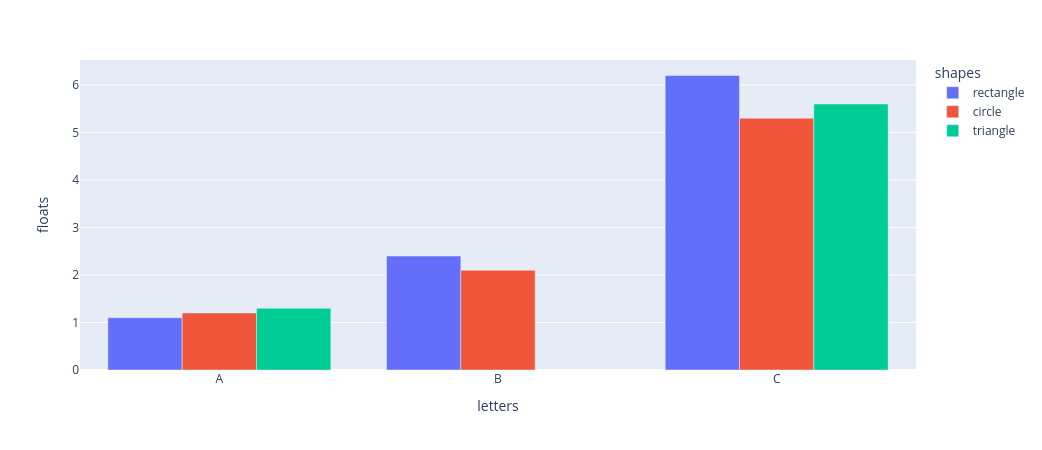
\includegraphics[width=7cm, height=7cm, keepaspectratio]{images/plots_12.png}
			\end{center}			
		\end{column}
	\end{columns}
\end{frame}

\begin{frame}{Összetett plotly express diagram létrehozása (\texttt{px\_app.py})}
	\begin{columns}
		\begin{column}{.5\textwidth}
			\begin{enumerate}
				\item Adathalmazok beolvasása, transzformációja és megfelelő formára hozása
				\item Változók létrehozása, amik megadják a szűrési kritériumokat: \texttt{year, indicator, grouper}
				\item Adathalmaz leszűrése a változók alapján
				\item A \texttt{px.scatter()} meghívása egy Dash objektum \texttt{Div} komponensén
			\end{enumerate}
		\end{column}
		\begin{column}{.5\textwidth}
			\begin{center}
				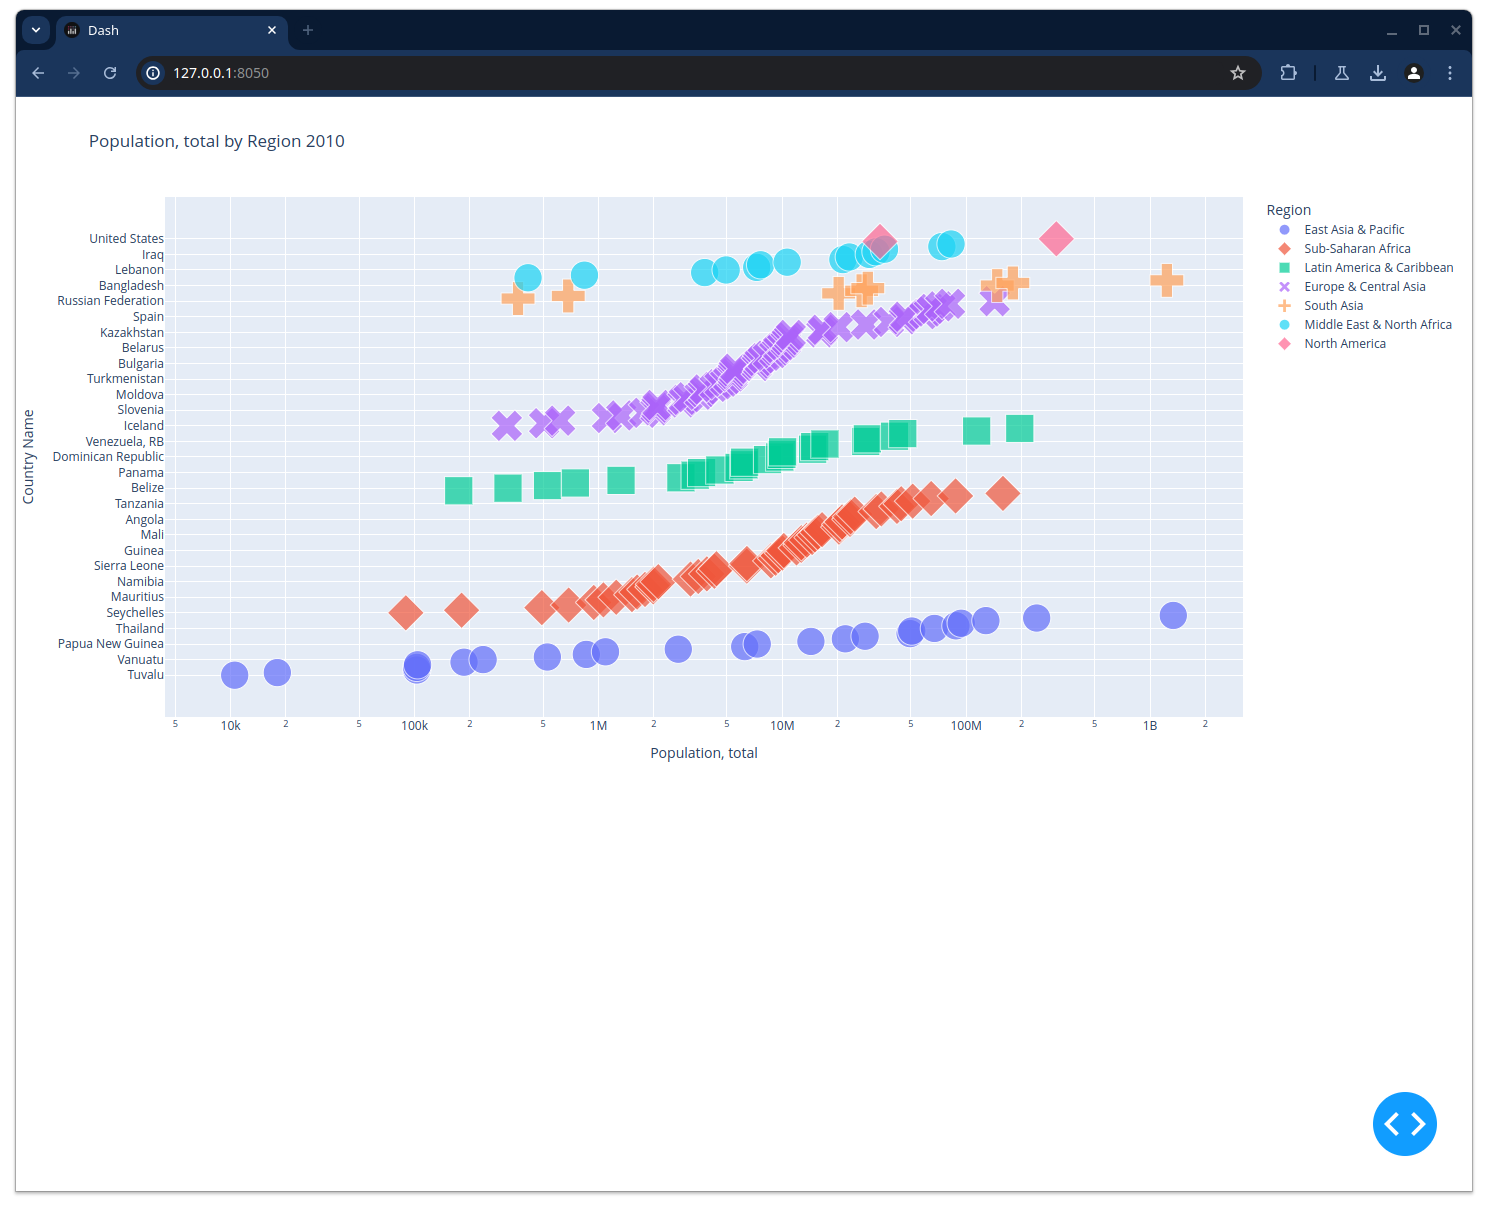
\includegraphics[width=7cm, height=7cm, keepaspectratio]{images/plots_13.png}
			\end{center}
		\end{column} 
	\end{columns}
\end{frame}

\section{Diagramok paraméterei}

\begin{frame}{}
	\tableofcontents[currentsection]
\end{frame}

\begin{frame}[fragile]{Fektetett oszlopdiagram}
	\begin{columns}
		\begin{column}{.5\textwidth}
			Vannak olyan esetek, amikor a tengelycímek hosszúak, ezért fontos a jó olvashatóság. Ebben az esetben a vízszintes oszlopdiagram a megfelelő választás.\par\smallskip
			Ehhez az \texttt{x} és \texttt{y} paramétereket meg kell cserélni és az \texttt{orientation='h'} paramétert be kell állítani:
			\begin{lstlisting}[language=python]
fig = px.bar(
	df, 
	x=gini, 
	y='Country Name', 
	title=' - '.join([gini, str(year)]), 
	orientation='h'
)
			\end{lstlisting}
		\end{column}
		\begin{column}{.5\textwidth}
			\begin{center}
				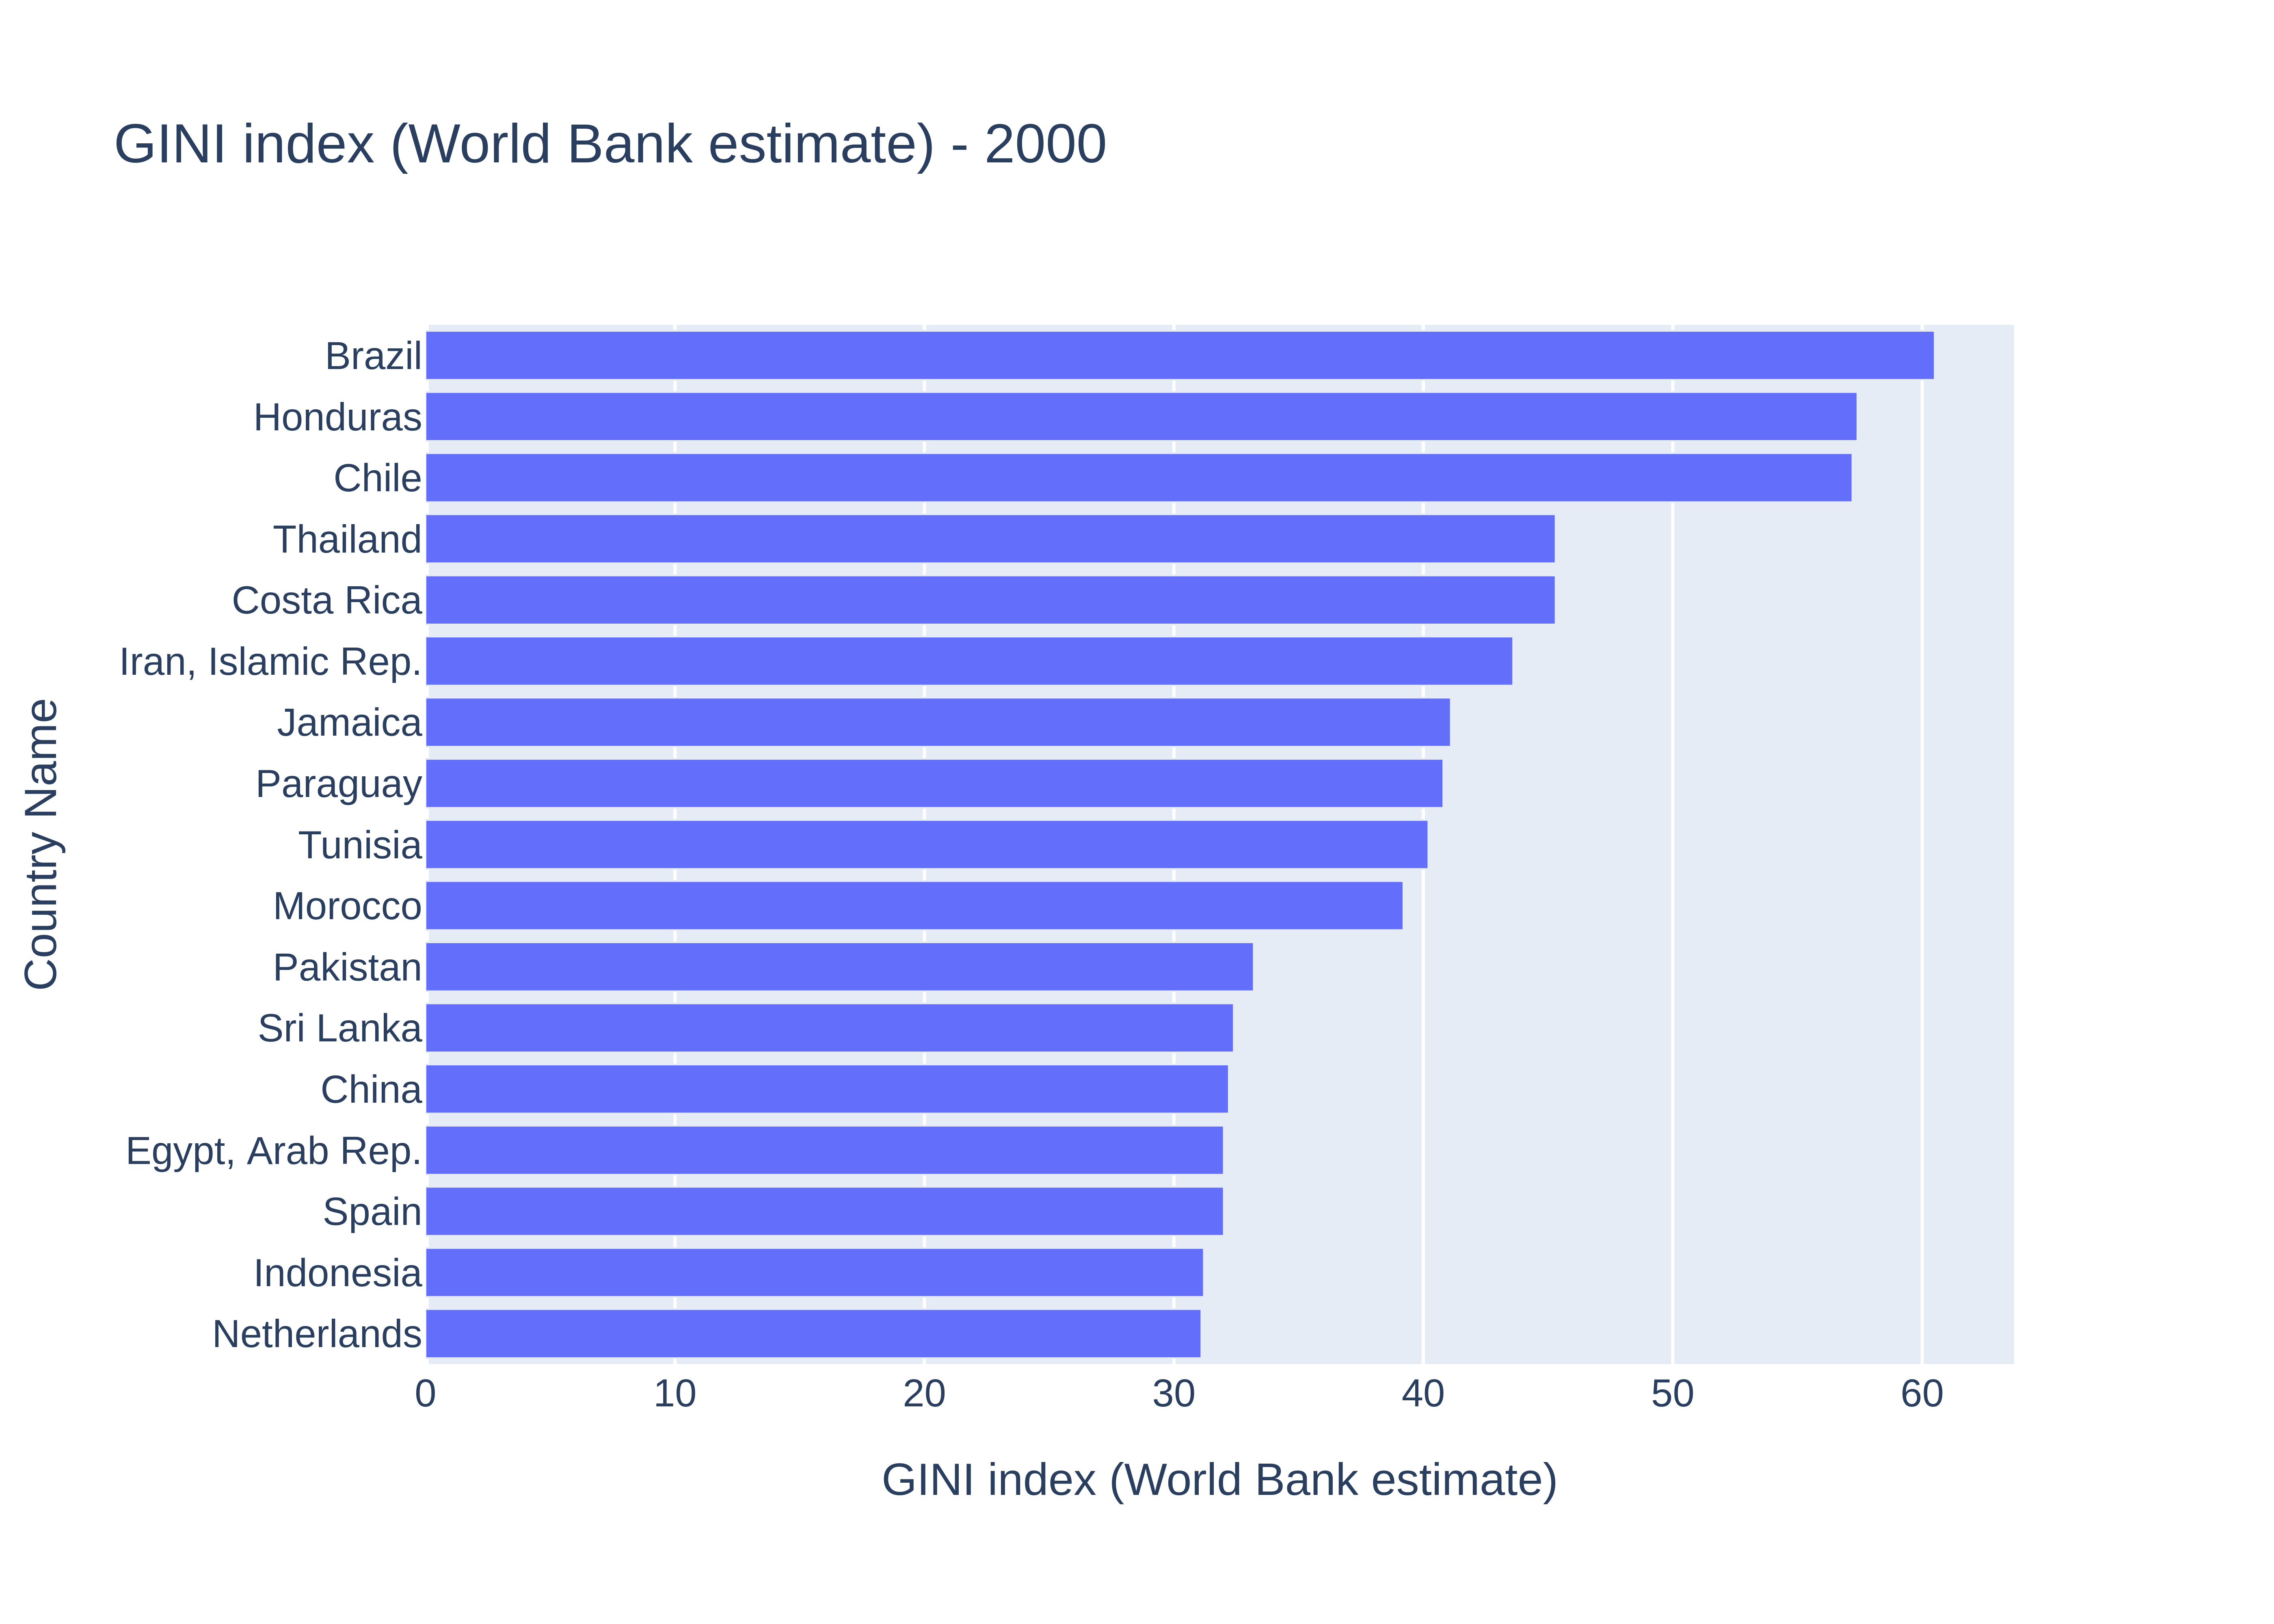
\includegraphics[width=7cm, height=7cm, keepaspectratio]{images/plots_15.png}
			\end{center}
		\end{column}
	\end{columns}
\end{frame}

\begin{frame}[fragile]{Dinamikus méretű oszlopdiagram}
	\begin{columns}
		\begin{column}{.5\textwidth}
			Alapértelmezés szerint a plotly express diagramok maximális méretének intervalluma $\left[20.2, 65.8\right]$. Ezt manuálisan is lehet állítani, de amikor kevés rekord van a diagram eltorzulhat.\par\smallskip
			Egy megoldás erre, ha országonként 20 pixellel nő meg a \texttt{height} paraméter.
			\begin{lstlisting}[language=python]
fig = px.bar(
	df,
	x=indicator,
	y='Country Name',
	title=' - '.join([gini, str(year)]),
	height=200 + (20 * n_countries),
	orientation='h',
)
			\end{lstlisting}
		\end{column}
		\begin{column}{.5\textwidth}
			\begin{center}
				\includegraphics[width=7cm, height=7cm, keepaspectratio]{images/plots_16.png}
			\end{center}
		\end{column}
	\end{columns}
\end{frame}

\begin{frame}{Oszlopmódok}
	\begin{columns}
		\begin{column}{.5\textwidth}
			Ugyanazt az oszlopdiagramot többféleképpen is meg lehet jeleníteni. Ennek a felelőse a \texttt{barmode} paraméter.\par\medskip
			\only<1>{
				\begin{block}{\texttt{relative}}
					Az oszlopok egymás mellett jelennek meg, és az értékek relatív különbségeit mutatják.
				\end{block}
			}
			\only<2>{
				\begin{block}{\texttt{group}}
					Az oszlopok csoportosítva jelennek meg, különböző kategóriák szerint.
				\end{block}
			}
			\only<3>{
				\begin{block}{\texttt{overlay}}
					Az oszlopok egymásra helyezve jelennek meg, átfedésben.
				\end{block}
			}
			\only<4>{
				\begin{block}{\texttt{stack}}
					Az oszlopok egymásra rakva jelennek meg, az értékek összeadódnak.
				\end{block}
			}
		\end{column}
		\begin{column}{.5\textwidth}
			\begin{center}
				\includegraphics<1>[width=7cm, height=7cm, keepaspectratio]{images/plots_19.png}
				\includegraphics<2>[width=7cm, height=7cm, keepaspectratio]{images/plots_20.png}
				\includegraphics<3>[width=7cm, height=7cm, keepaspectratio]{images/plots_21.png}
				\includegraphics<4>[width=7cm, height=7cm, keepaspectratio]{images/plots_22.png}
			\end{center}
		\end{column}
	\end{columns}
\end{frame}

\begin{frame}[fragile]{Diagramok szétbontása felületekre}
	\begin{columns}
		\begin{column}{.5\textwidth}
			Szétbontással új dimenziókat lehet felvenni egy műszerfalra. Ki lehet választani egy jellemzőt, ami mentén a szeletelés történik. A megfelelő paraméterek erre a plotly express könyvtárban a \texttt{facet\_col} és \texttt{facet\_row} attól függően, hogy új oszlop vagy sor fog létrejönni a diagramban. \par\medskip
			\begin{lstlisting}[language=python]
fig = px.bar(df, x='year', y=gini, facet_row='Country Name')				
			\end{lstlisting}
		\end{column}
		\begin{column}{.5\textwidth}
			\begin{center}
				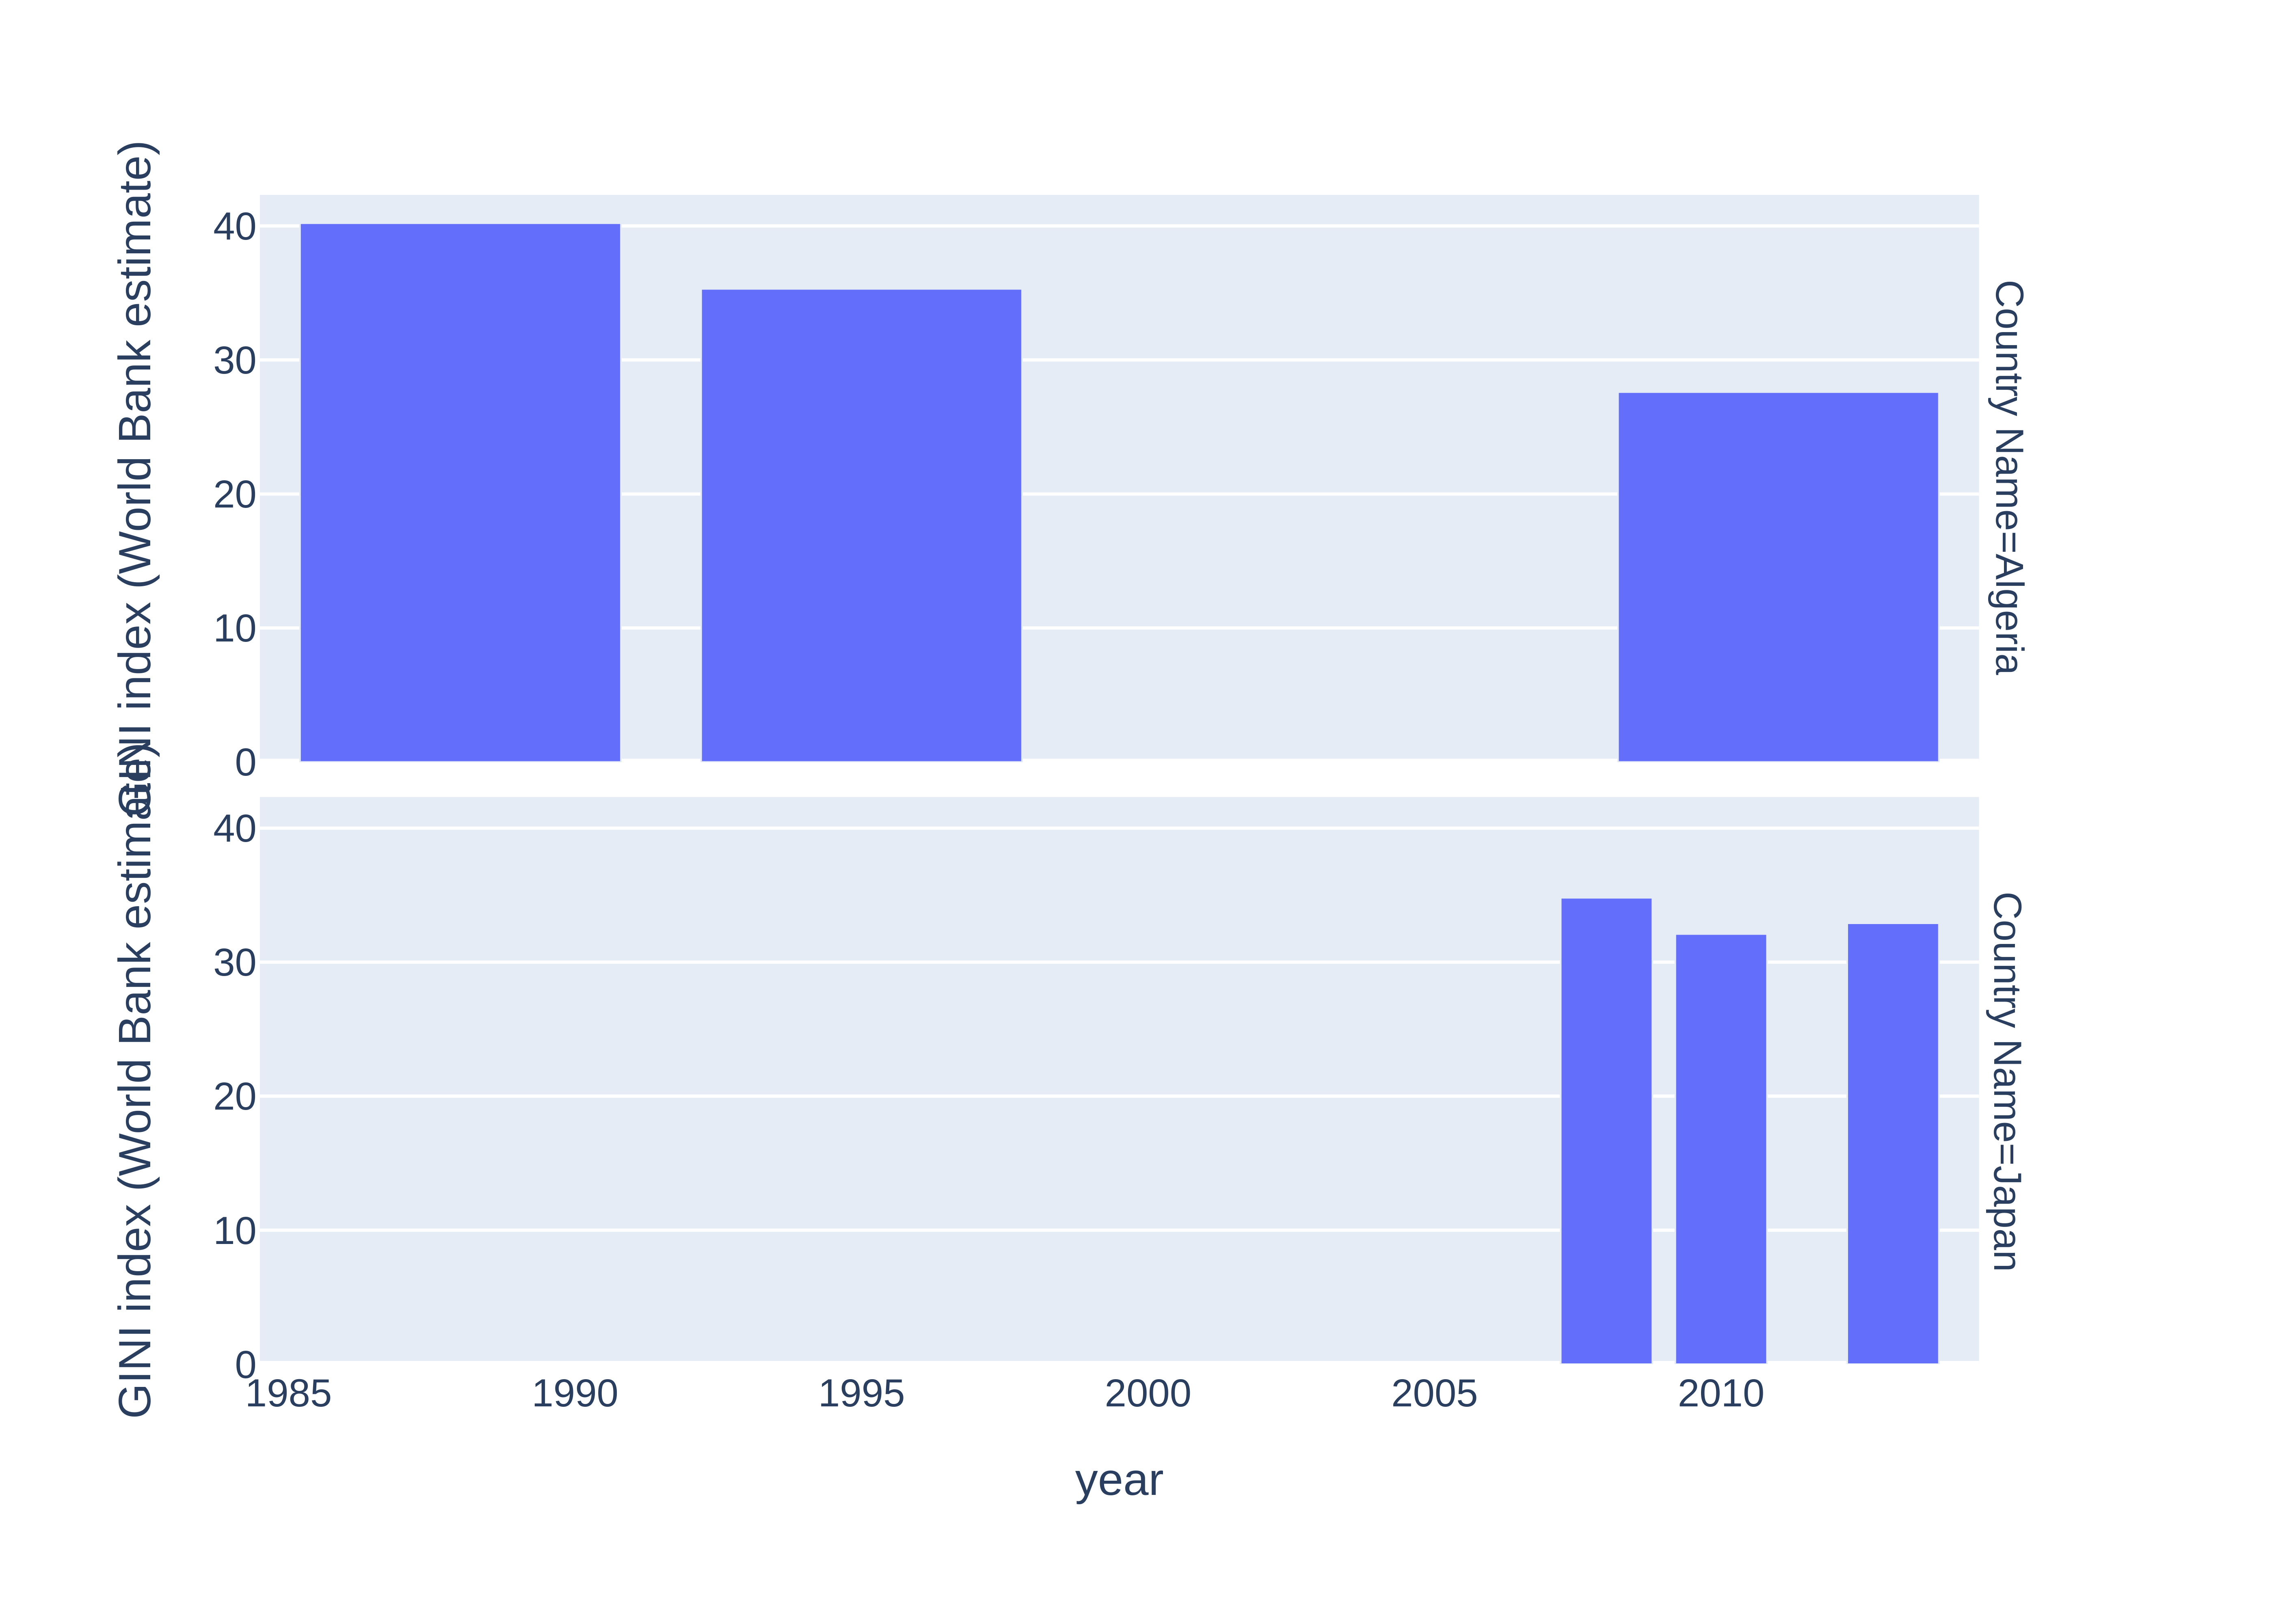
\includegraphics[width=7cm, height=7cm, keepaspectratio]{images/plots_23.png}
			\end{center}
		\end{column}
	\end{columns}
\end{frame}

\section{Dinamika diagramokkal}

\begin{frame}{}
	\tableofcontents[currentsection]
\end{frame}

\begin{frame}[fragile]{Legnépesebb országok régiónként}
	\begin{columns}
		\begin{column}{.5\textwidth}
			Egy legördülő listán ki lehet választani az évek közül a megfelelőt, ez elindít egy callback függvényt, ami egy \texttt{dcc.Graph} objektun \texttt{figure} adattagját frissíti egy plotly express diagrammal.
			\begin{lstlisting}[language=python]
dcc.Dropdown(
	id='year_dropdown',
	value='2010',
	options=[{'label': year, 'value': str(year)} for year in range(1974, 2019)]
),
...
dcc.Graph(id='population_chart'),				
			\end{lstlisting}
		\end{column}
		\begin{column}{.5\textwidth}
			\begin{lstlisting}[language=python]
@param_app.callback(
	Output('population_chart', 'figure'),
	Input('year_dropdown', 'value')
)
def plot_countries_by_population(year):
	fig = go.Figure()
	year_df = population_df[['Country Name', year]].sort_values(year, ascending=False)[:20]
	fig.add_bar(x=year_df['Country Name'], y=year_df[year])
	fig.layout.title = f'A húsz legnépesebb ország - {year}'
	return fig				
			\end{lstlisting}
		\end{column}
	\end{columns}
\end{frame}

\begin{frame}[fragile]{Többváltozós legördülő lista}
	\begin{columns}
		\begin{column}{.5\textwidth}
			A \texttt{Dropdown} komponensnek van egy extra, opcionális paramétere, a \texttt{multi}, ami egy logikai változót vár el értékként, és ha be van kapcsolva lehetővé teszi több érték kiválasztását egy változóból.\par\medskip
			\begin{lstlisting}[language=python]
dcc.Dropdown(
	id='gini_country_dropdown', 
	multi=True,
	options=[{'label': country, 'value': country} for country in gini_df['Country Name'].unique()]
),				
			\end{lstlisting}
		\end{column}
		\begin{column}{.5\textwidth}
			\begin{center}
				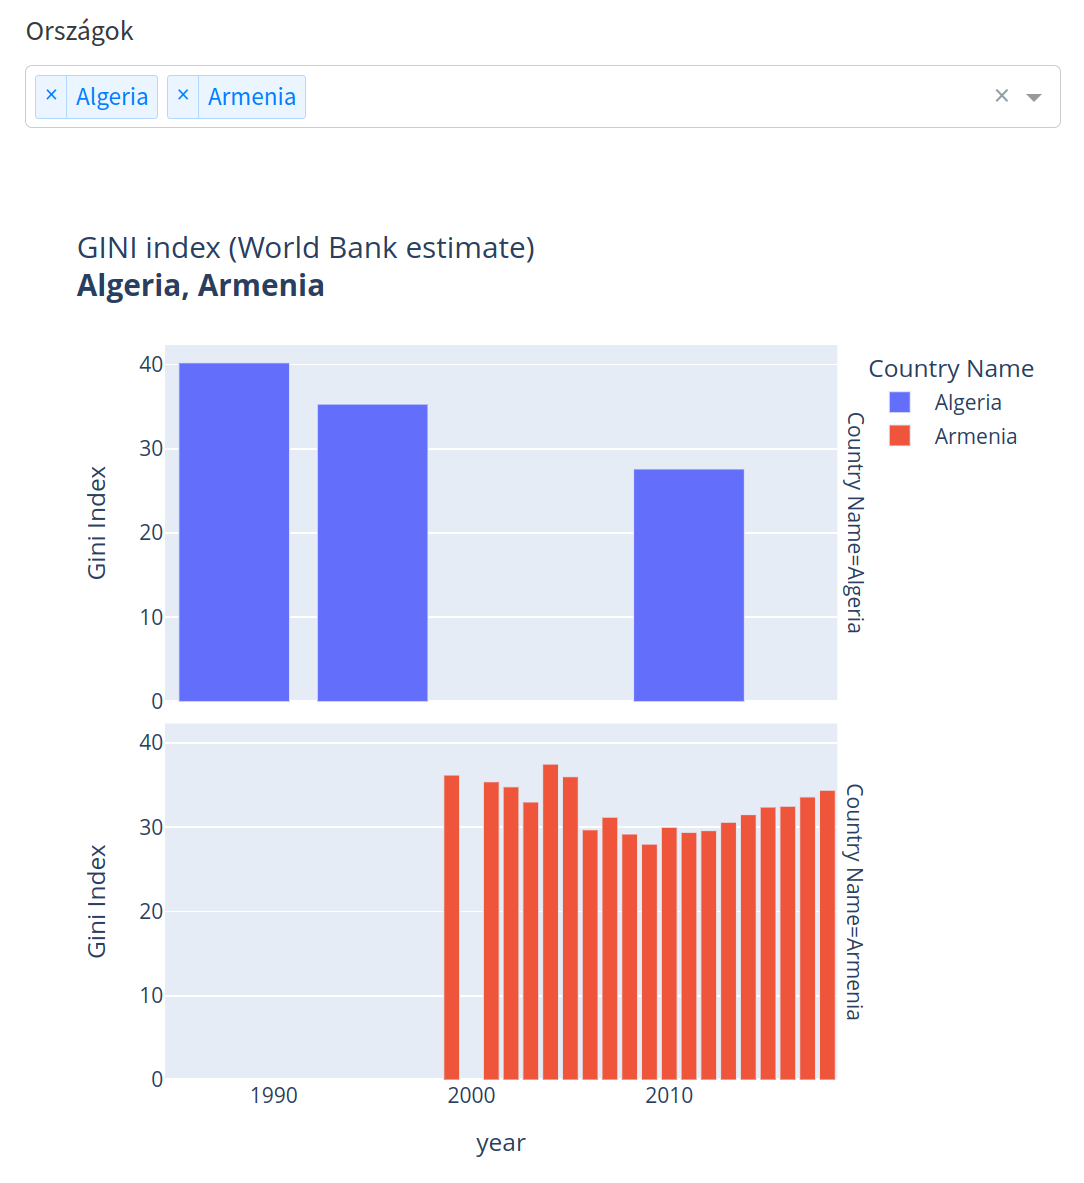
\includegraphics[width=7cm, height=7cm, keepaspectratio]{images/plots_24.png}
			\end{center}			
		\end{column}
	\end{columns}
\end{frame}

\begin{frame}[fragile]{Helykitöltő szöveg legördülő listákhoz}
	Egy további opcionális paramétere a \texttt{Dropdown} objektumoknak a \texttt{placeholder}, amivel lehetséges helykitöltő szöveget hozzáadni a legördülő listához.\par\smallskip
	Ezzel megjelenít egy szöveget, ami azelőtt látszik, hogy a felhasználó belekattintana dobozba.
	\begin{columns}
		\begin{column}{.5\textwidth}
			\begin{lstlisting}[language=python]
dcc.Dropdown(
	id='gini_country_dropdown',
	placeholder='Válasszon egy vagy több országot',
	multi=True,
	options=[{'label': country, 'value': country} for country in gini_df['Country Name'].unique()]
),				
			\end{lstlisting}
		\end{column}
		\begin{column}{.5\textwidth}
			\begin{center}
				
\includegraphics[width=7cm, height=7cm, keepaspectratio]{images/plots_26.png}
			\end{center}
		\end{column}
	\end{columns}
\end{frame}

\begin{frame}[fragile]{Elrendezés komponensek újrafelhasználása}
	\begin{columns}
		\begin{column}{.5\textwidth}
			Egy python szkriptben inicializált \texttt{layout} változót lehetséges egy másik szkriptben importálni.\par\medskip
			Ebben az esetben a \texttt{layout.children} komponenst egy listaként kell átvenni, és hozzá kell fűzni az aktuális szkript elrendezés definíciójához.
		\end{column}
		\begin{column}{.5\textwidth}
			\begin{lstlisting}[language=python]
app.layout = html.Div([
	*app_v2_3.app.layout.children[:-1],
	dbc.Row([
		...	
	]),
	app_v2_3.app.layout.children[-1]
])				
			\end{lstlisting}			
		\end{column}
	\end{columns}
\end{frame}

\begin{frame}[fragile]{A lista kicsomagolás operátor}
	\begin{columns}
		\begin{column}{.5\textwidth}
			Az előző példában a listára értelmezett \texttt{*} operátor a python nyelvben arra használható, hogy egy lista értékeit kicsomagolja valamilyen argumentumban vagy másik adatstruktúrában.
			\begin{lstlisting}[language=python]
In [1]: a = [1, 2, 3]
In [2]: b = 5
In [3]: [*a, 4, b]
Out[3]: [1, 2, 3, 4, 5]
			\end{lstlisting}
		\end{column}
		\begin{column}{.5\textwidth}
			Ez a funkcionalitás akkor használatos, ha arra van szükség, hogy egy függvény tetszőleges számú paramétert legyen képes átvenni:
			\begin{lstlisting}[language=python]
def f(*argv):
	...
	
f('Hello', 'World')
			\end{lstlisting}
			Abban az esetben ha nevesített argumentumokra van szűkség a \texttt{**} operátor teszi ezt lehetővé:
			\begin{lstlisting}[language=python]
def f(**kwargs):
	...

f(school='bge', spec='data')
			\end{lstlisting}
		\end{column}
	\end{columns}
\end{frame}

\begin{frame}[fragile]{Callback függvények újrafelhasználása}
	\begin{columns}
		\begin{column}{.5\textwidth}
			Callback függvényeket is lehetséges felhasználni szkriptek között, viszont ennek az eljárása eltér az elrendezés komponensek újrafelhasználásának módjától.\par\smallskip
			Ahhoz, hogy egy alkalmazásba be lehessen importálni egy másik alkalmazás callback függvényeit, a definíció helyén egy külső függvénybe kell ezeket beágyazni, majd ezt a függvényt később meghívni egy paraméterezett \texttt{Dash} alkalmazás objektummal.
		\end{column}
		\begin{column}{.5\textwidth}
			\begin{lstlisting}[language=python]
def register_callbacks(param_app):
	@param_app.callback(
		...
	)
	def callback1(...):
		...
	
	@param_app.callback(
		...
	)
	def callback2(...):
		...				
			\end{lstlisting}
			A meghívás egy másik alkalmazásból:
			\begin{lstlisting}[language=python]
import app_v2_1

app = dash.Dash(__name___)
...
app_v2_1.register_callbacks(app)
			\end{lstlisting}
		\end{column}
	\end{columns}
\end{frame}

\end{document}





